
%% paper.tex
%% for ISORC 2016
%% 2016/11/29
%% by Takuro Yamamoto

\documentclass[conference]{IEEEtran/IEEEtran}
% Some Computer Society conferences also require the compsoc mode option,
% but others use the standard conference format.
%
% If IEEEtran.cls has not been installed into the LaTeX system files,
% manually specify the path to it like:
% \documentclass[conference]{../sty/IEEEtran}

% Package List
%\usepackage[dvips]{graphics}
\usepackage[dvipdfmx]{graphicx}
\usepackage{amssymb}
\usepackage{float}
\usepackage{enumerate,cite,url}
\usepackage{listings,jlisting}
\lstset{%
    language={c},%
    basicstyle={\footnotesize\ttfamily},%
    identifierstyle={\footnotesize},%
    commentstyle={\footnotesize\itshape},%
    keywordstyle={\footnotesize},%\bfseries},%
    ndkeywordstyle={\footnotesize},%
    stringstyle={\footnotesize\it},
    frame={tb},
    breaklines=true,
    columns=[l]{fullflexible},%
    numbers=left,%
    xrightmargin=0zw,%
    xleftmargin=3zw,%
    numberstyle={\scriptsize},%
    stepnumber=1,
    numbersep=1zw,%
    lineskip=-0.5ex%
}

% *** Do not adjust lengths that control margins, column widths, etc. ***
% *** Do not use packages that alter fonts (such as pslatex).         ***
% There should be no need to do such things with IEEEtran.cls V1.6 and later.
% (Unless specifically asked to do so by the journal or conference you plan
% to submit to, of course. )


% correct bad hyphenation here
\hyphenation{op-tical net-works semi-conduc-tor}


\begin{document}
%
% paper title
% Titles are generally capitalized except for words such as a, an, and, as,
% at, but, by, for, in, nor, of, on, or, the, to and up, which are usually
% not capitalized unless they are the first or last word of the title.
% Linebreaks \\ can be used within to get better formatting as desired.
% Do not put math or special symbols in the title.
\title{TINET+TECS: Component-Based TCP/IP Protocol Stack for Embedded Systems}


% author names and affiliations
% use a multiple column layout for up to three different
% affiliations
% \author{
% \IEEEauthorblockN{Takuro Yamamoto}
% \IEEEauthorblockA{Graduate School of Engineering Science\\Osaka University}
% \and
% \IEEEauthorblockN{Takuma Hara}
% \IEEEauthorblockA{Graduate School of Information Science\\Nagoya University}
% \and
% \IEEEauthorblockN{Takuya Ishikawa}
% \IEEEauthorblockA{Graduate School of Information Science\\Nagoya University}
% \and
% \IEEEauthorblockN{Hiroshi Oyama}
% \IEEEauthorblockA{OKUMA Corporation}
% \and
% \IEEEauthorblockN{Hiroaki Takada}
% \IEEEauthorblockA{Graduate School of Information Science\\Nagoya University}
% \and
% \IEEEauthorblockN{Takuya Azumi}
% \IEEEauthorblockA{Graduate School of Engineering Science\\Osaka University}
% }

% conference papers do not typically use \thanks and this command
% is locked out in conference mode. If really needed, such as for
% the acknowledgment of grants, issue a \IEEEoverridecommandlockouts
% after \documentclass

% for over three affiliations, or if they all won't fit within the width
% of the page, use this alternative format:
% 
\author{
\IEEEauthorblockN{
Takuro Yamamoto\IEEEauthorrefmark{1},
Takuma Hara\IEEEauthorrefmark{2},
Takuya Ishikawa\IEEEauthorrefmark{2}, 
Hiroshi Oyama\IEEEauthorrefmark{3},
Hiroaki Takada\IEEEauthorrefmark{2} and
Takuya Azumi\IEEEauthorrefmark{1}}
\IEEEauthorblockA{\IEEEauthorrefmark{1}Graduate School of Engineering Science, Osaka University}
\IEEEauthorblockA{\IEEEauthorrefmark{2}Graduate School of Information Science, Nagoya University}
\IEEEauthorblockA{\IEEEauthorrefmark{3}OKUMA Corporation}
}

% use for special paper notices
%\IEEEspecialpapernotice{(Invited Paper)}

% make the title area
\maketitle

\setcounter{topnumber}{5}       % ページ上部の図表は 5 個まで
\def\topfraction{1.00}          % ページの上 1.00 まで図表で占めて可
\setcounter{bottomnumber}{5}    % ページ下部の図表は 5 個まで
\def\bottomfraction{1.00}       % ページの下 1.00 まで図表で占めて可
\setcounter{totalnumber}{10}    % ページあたりの図表は 10 個まで
\def\textfraction{0.04}         % ページうち本文が占める割合の下限

% As a general rule, do not put math, special symbols or citations
% in the abstract
\begin{abstract}

% Embedded systems are applied to Internet of Things (IoT), and the high productivity of embedded network software is required.
High productivity embedded network software is required to run embedded systems within the Internet of Things (IoT).
Tomakomai InterNETworking (TINET) is a Transmission Control Protocol/Internet Protocol (TCP/IP) protocol stack for use in embedded systems.
Although TINET is a compact protocol stack, it comprises many complex source codes and is difficult to maintain, extend, and analyze.
To improve scalability and configurability, this paper proposes TINET componentized with the Toyohashi Open Platform for Embedded Real-time Systems (TOPPERS) embedded component system (TINET+TECS), a component-based TCP/IP protocol stack for embedded systems.
This component-based TINET offers software developers high productivity through variable network buffer sizes and the ability to add or remove TCP (or UDP) functionality.
TINET+TECS utilizes a dynamic TECS component connection method to satisfy the original TINET specifications.
The results of an experimental comparison between the proposed component-based and original TINETs show that the execution time and memory consumption overhead are reduced and the configurability is improved.

\end{abstract}

% no keywords

% For peer review papers, you can put extra information on the cover
% page as needed:
% \ifCLASSOPTIONpeerreview
% \begin{center} \bfseries EDICS Category: 3-BBND \end{center}
% \fi
%
% For peerreview papers, this IEEEtran command inserts a page break and
% creates the second title. It will be ignored for other modes.
\IEEEpeerreviewmaketitle

\section{Introduction}
\label{sec:Introduction}

The Internet of Things (IoT) is an essential next evolutionary step for the Internet \cite{par:IoTIndustries} \cite{par:IoTComputing} in which various items and platforms, for example, wearable devices, smart devices, and smart homes, will be connected via the Internet to further enrich people's lives.
However, as the IoT uses embedded systems such as data sensors and controlling actuators as elemental constituents, it is often not practical to implement the same Transmission Control Protocol/Internet Protocol (TCP/IP) protocol stacks used by traditional computing systems because embedded systems face restrictions in terms of, for example, low memory capacity.

Tomakomai InterNETworking (TINET) is a compact TCP/IP protocol stack for embedded systems \cite{url:TINET}.
As TINET supports functionalities such as a minimum copy frequency and the elimination of dynamic memory control, it requires significantly reduced memory for its TCP/IP protocol stack and is therefore suitable for embedded systems.
However, TINET comprises many complex source codes, i.e., it contains many files and defines many macros, which can be problematic for software developers seeking to maintain, extend, and analyze the software.
Thus, embedded network software is required for high productivity and quality.

One approach to improving software productivity is component-based development, a design technique that can be applied in reusable software development for embedded systems \cite{par:Crnkovic}\cite{par:CBD} such as TECS \cite{par:TECS} \cite{par:hr-tecs}, AUTOSAR \cite{url:AUTOSAR}, or SaveCCM \cite{par:SAVEapproach}.
Component-based systems are flexible to software extension and specification changes.

This paper proposes a component-based TCP/IP protocol stack for embedded systems--TINET componentized with the Toyohashi Open Platform for Embedded Real-time Systems (TOPPERS) embedded component system (TINET+TECS)--to improve the configurability and scalability of TCP/IP software.
Because it is a component system suitable for embedded systems, TECS \cite{par:TECS} \cite{par:hr-tecs} is used to componentize TINET in the proposed protocol stack.
As TECS supports static configurations that statically define component behaviors and interconnections, it can optimize the componentization overhead.

In addition to satisfying the original TINET specifications, the proposed framework utilizes the TECS dynamic connection capability to dynamically switch component bindings.
Although general TCP/IP protocol servers dynamically process requested ports, i.e., Hypertext Transfer Protocol (HTTP, port: 80) and Hypertext Transfer Protocol Secure (HTTPS, port: 443), embedded systems are restricted in their dynamic processing ability owing to strict memory constraints.
TINET supports the static generation of Communication Endpoints (CEPs) and Reception Points (REPs), which are similar to sockets.
As TINET+TECS, like TINET, statically generates components and dynamically combines them in the same manner, TINET+TECS reduces the dynamic increase of memory consumption.

In the proposed framework, software applications can be developed using both TECS method and existing methods.
Software applications can be developed as TECS components because TINET+TECS is a component-based framework.
Furthermore, TECS supports the use of an adapter to call TECS component functions from non-TECS codes, which allows for the use of existing TCP/IP applications without modification.

This paper evaluates the overheads of execution time and memory consumption and the amount of code line changes needed to add and remove functionalities in order to improve configurability with small overheads.
Furthermore, the advantages of dynamic connection in terms of the memory consumption and low overhead of the TECS adapter are demonstrated.

{\bf Contributions:} This paper provides the following contributions:

\begin{enumerate}

    \item {\bf Improve configurability}\mbox{}\\
        Because TINET+TECS is a component-based system, its software can flexibly change as system's configuration by, for example, resizing network buffer, adding/removing TCP (or UDP) functionality, or supporting either IPv4 or IPv6.
        In addition, the use by TINET+TECS of individual component diagrams enables visualization of an entire system.

    \item {\bf Dynamic connection method}\mbox{}\\
        Dynamically switching the binding of components, that is, switching between a TINET communication endpoint and REP, realizes a TCP/IP protocol stack for an embedded system.
        
    \item {\bf Support legacy codes}\mbox{}\\
        TINET+TECS can be applied to existing applications because TECS supports the ability of the adapter to call TECS functions from C codes. 
    % \item {\bf Software visualization}

\end{enumerate}

{\bf Organization}: The remainder of this paper is organized as follows.
Section \ref{sec:System Model} introduces the system model and its basic technologies, i.e., TINET and TECS.
Section \ref{sec:Design and Implementation} describes the design and implementation of the proposed framework.
Section \ref{sec:Evaluation} evaluates the proposed framework and demonstrates its advantages.
Related work is discussed in Section \ref{sec:Related Work}.
Conclusions and suggestions for future work are presented in Section \ref{sec:Conclusion}.


\section{System Model}
\label{sec:System Model}

This section describes the system model of TINET+TECS, including basic technologies such as TINET and TECS.
A system model of the proposed framework is shown in Fig. \ref{fig:SystemModel}.
TINET+TECS is a component-based TCP/IP protocol stack in which the TCP output task (tTCPOutput) and Ethernet input task (tEhternetInput) are implemented as TECS components.
CEPs and REPs (Section \ref{sec:TINET}), which are also implemented as TECS components, dynamically switch bindings using the TECS method.
Moreover, the TECS adapter supports the legacy codes for existing TCP/IP applications.

\begin{figure}[t]
    \centering
    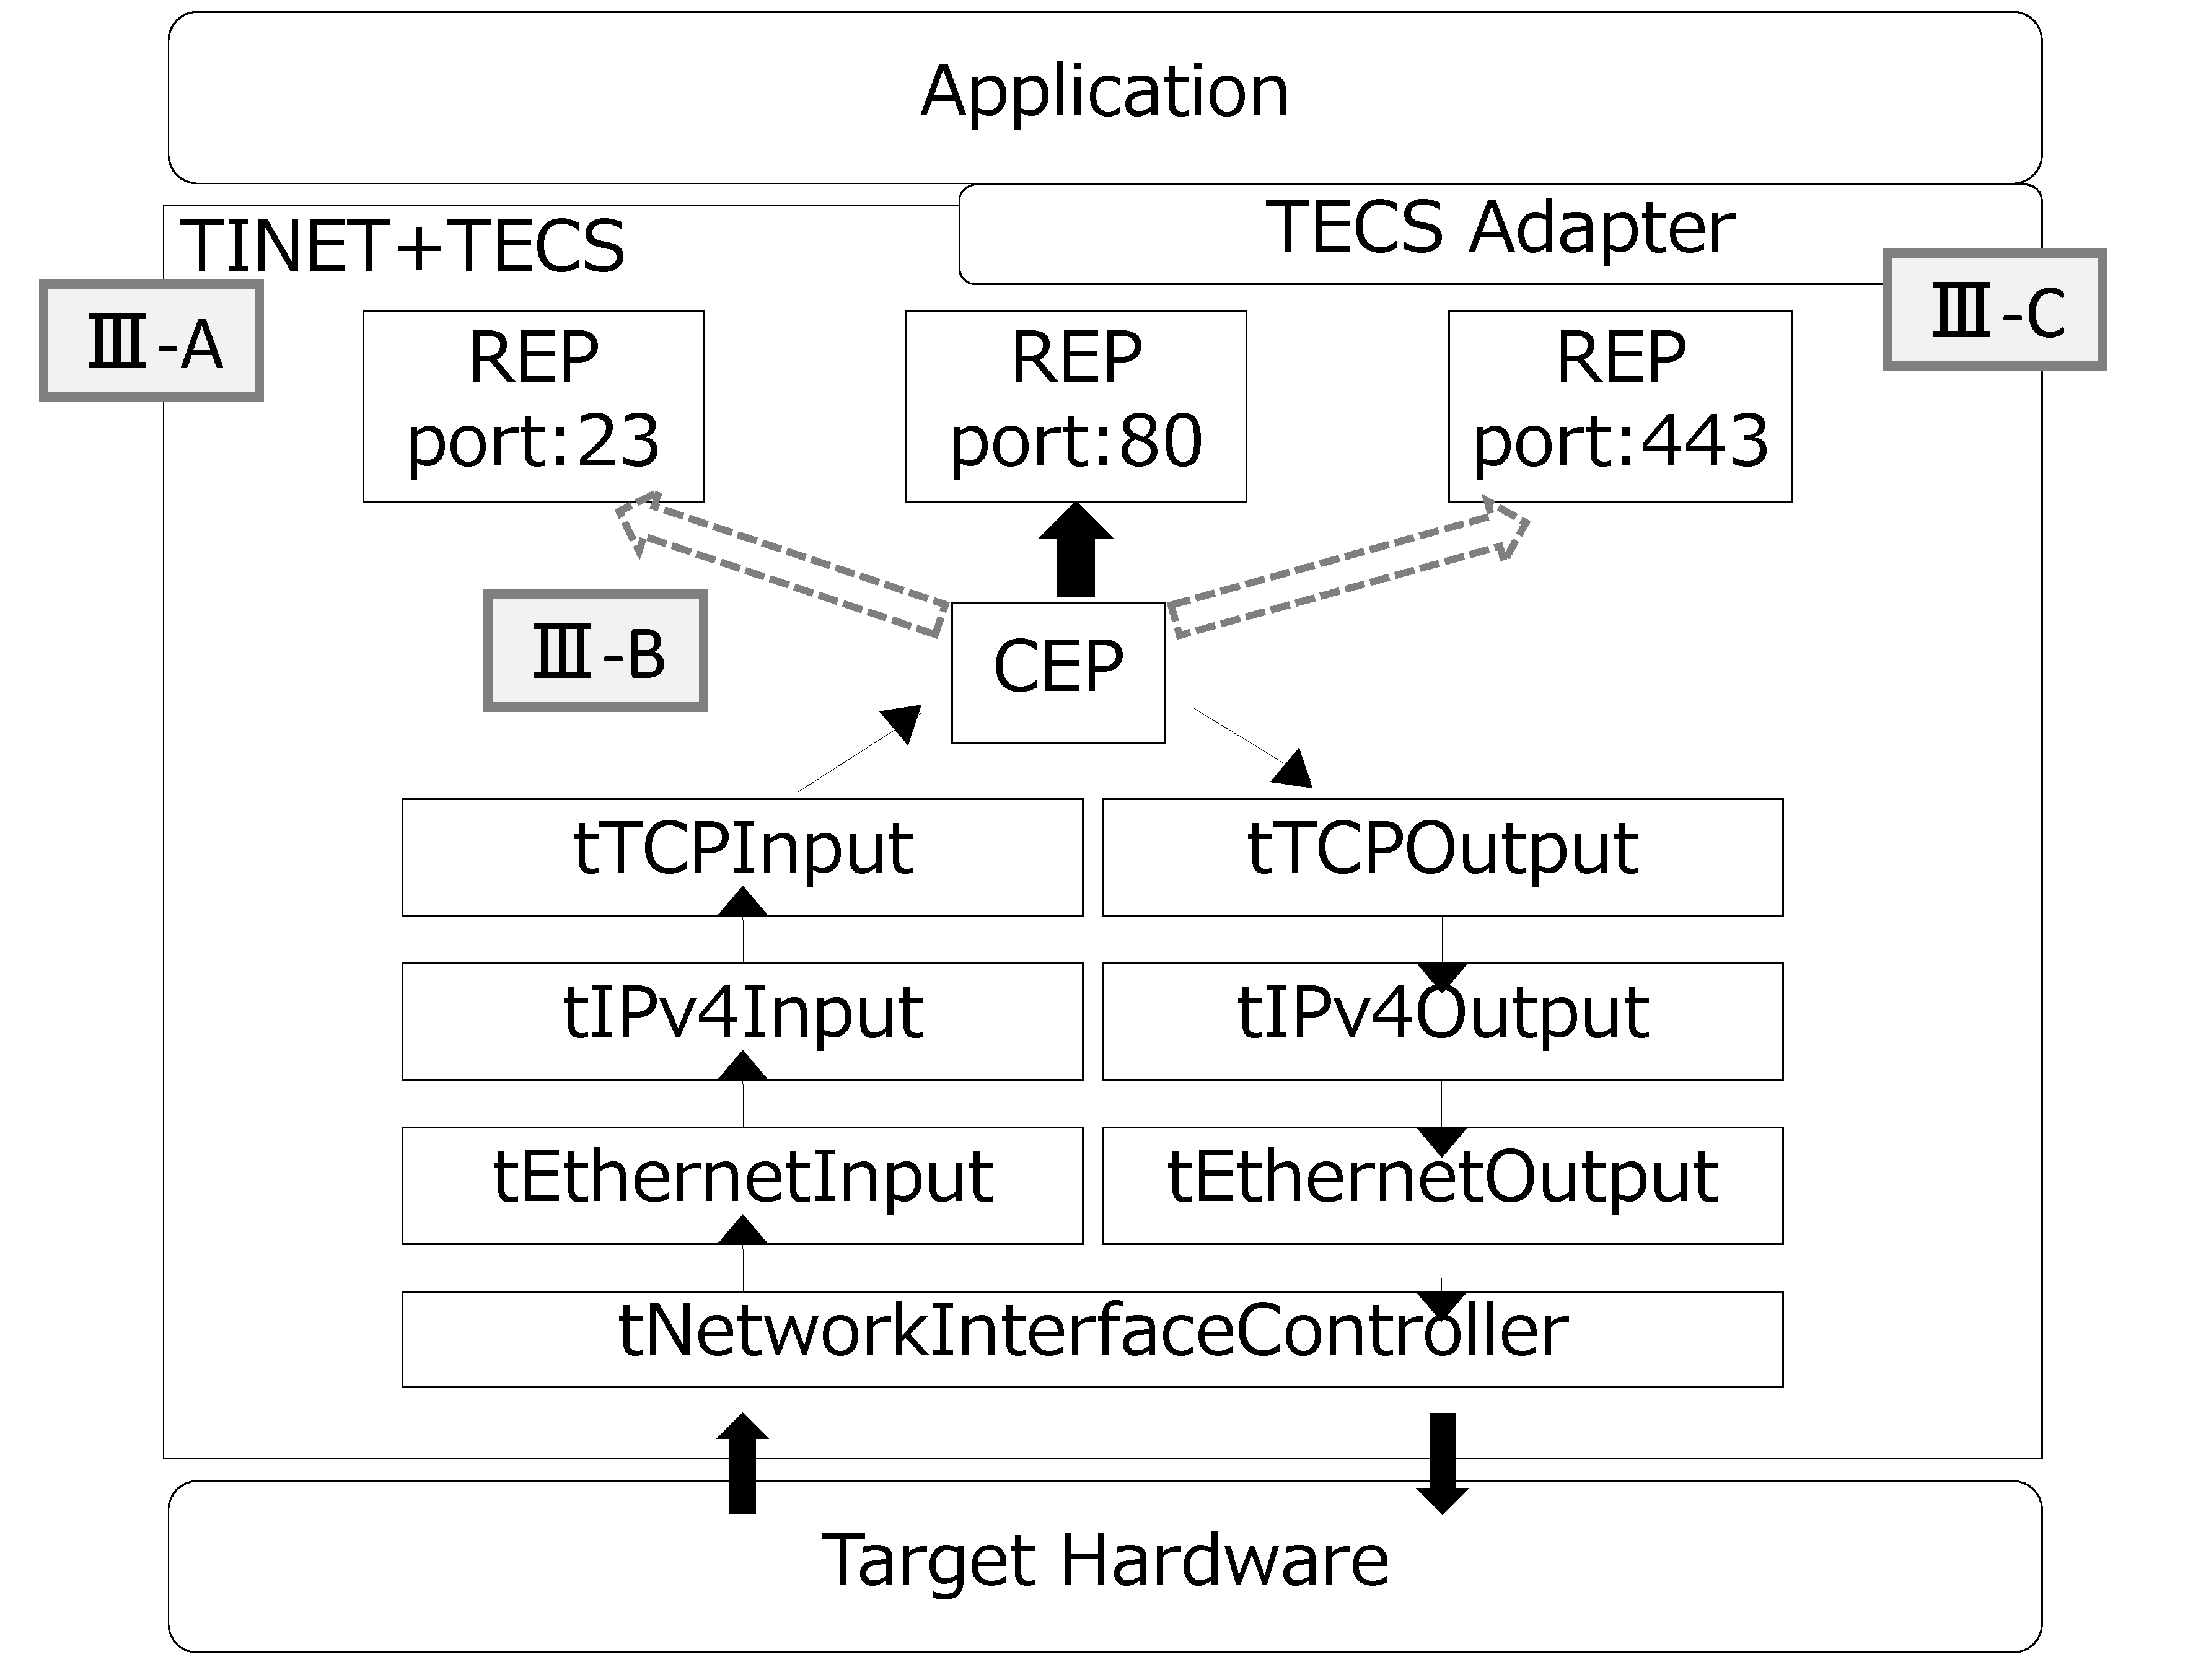
\includegraphics[width=8.0cm,clip]{figure/SystemModel.pdf}
    \caption{System model of TINET+TECS}
    \label{fig:SystemModel}
\end{figure}

\subsection{TINET}
\label{sec:TINET}

TINET is a compact TCP/IP protocol stack for embedded systems based on the ITRON\footnote{ITRON is a realtime operating system (RTOS) developed by the TRON project.} TCP/IP API Specification \cite{url:ITRON_TCP/IP_API_Spec}, developed by the TOPPERS Project \cite{url:TOPPERS}.
TINET has been released as an open-source tool.

To satisfy restrictions for embedded systems in terms of, for example, memory capacity, size, and power consumption, TINET supports the following functions:

\begin{itemize}
    \item minimum copy frequency,
    \item elimination of dynamic memory control,
    \item asynchronous interfacing,
    \item error detailing per API.
\end{itemize}

\subsubsection{Overview}

TINET runs as middleware on TOPPERS/ASP3 \cite{par:ASP3} \cite{url:ASP3}, a real-time kernel based on $\mu$ITRON \cite{par:microITRON}.
As it is compatible with TOPPERS RTOS, TINET also supports other RTOSs such as TOPPERS/ASP and TOPPERS/JSP.

Fig. \ref{fig:TINETHierarchyDiagram} shows the hierarchy diagram of TINET and TOPPERS/ASP3.
% TINET supports ITRON TCP/IP API such as {\it tcp\_snd\_buf}, {\it tcp\_rcv\_buf}, {\it udp\_snd\_buf}, and {\it udp\_rcv\_buf}.
Users transmit and receive data using a Communication End Point (CEP), an interface that functions like a socket.
In the transmission process, headers are attached to the data body passed to the CEP at each protocol layer before the data are transmitted from the network device.
In the reception process, the headers of the data bodies received by the network device are analyzed at each protocol layer, and the data are then passed to the CEP.

A TCP reception point called the REP stands by to receive connection requests from the partner side.
The REP has an IP address ({\it myaddr}) and a port number ({\it myportno}) as attributes and performs functions such {\it bind()} and {\it listen()}.

In TINET, the amount of data copying between each protocol layers is minimized.
In standard computing systems, the TCP/IP protocol stack has large overheads in terms of execution time and memory consumption because the data are copied at each protocol layer.
To solve this problem, TINET does passes the pointer of the data buffer between each protocol layer instead of performing data copying.

\begin{figure}[t]
    \centering
    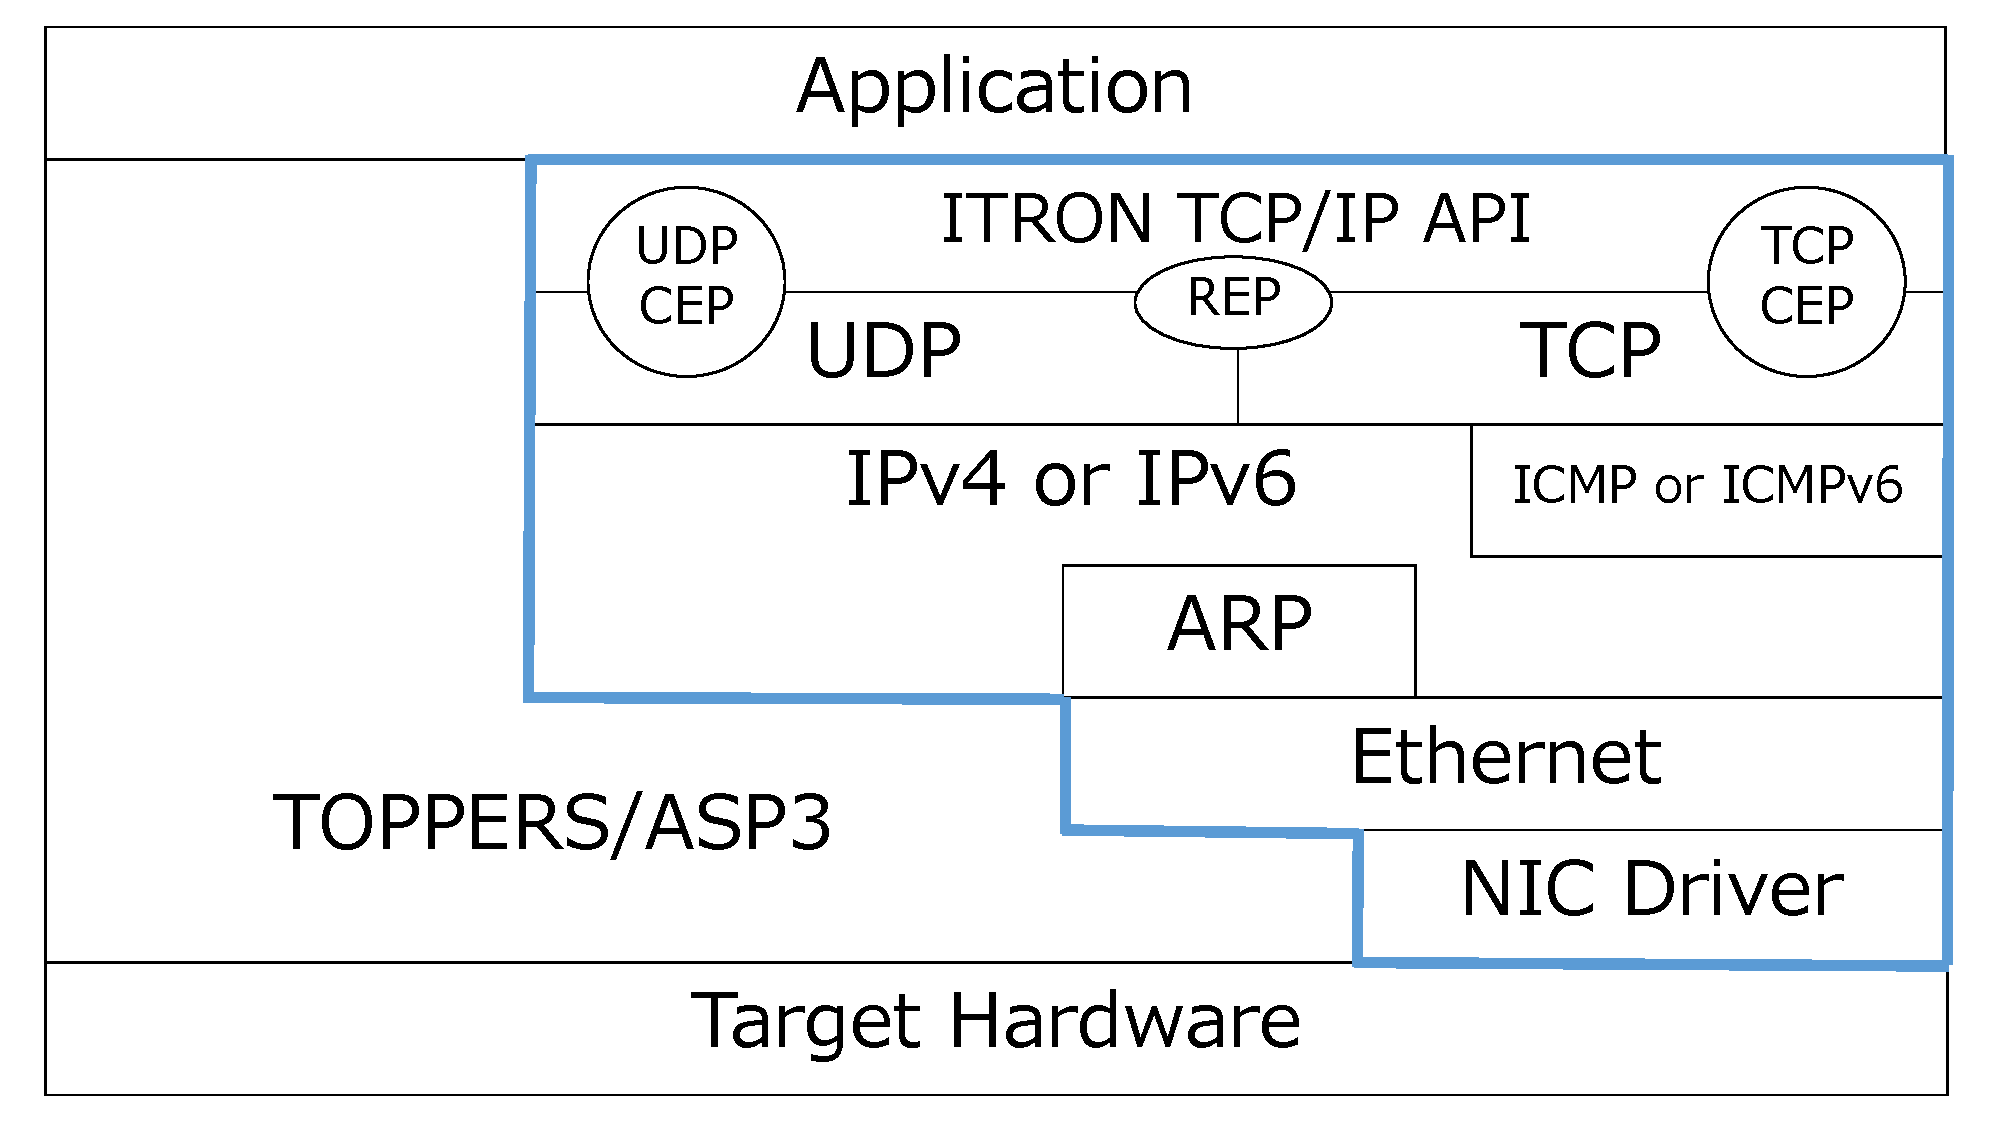
\includegraphics[width=8.0cm,clip]{figure/TINETHierarchyDiagram.pdf}
    \caption{TINET and TOPPERS/ASP3 hierarchy diagrams}
    \label{fig:TINETHierarchyDiagram}
\end{figure}

\subsection{TECS}
\label{sec:TECS}

TECS is a component system suitable for embedded systems that can increase productivity and reduce development costs based on the improved reusability of software components.
TECS also provides component diagrams that can help developers visualize the overall structure of a system.

In TECS, component deployment and composition are performed statically, and as a consequently, component connection does not incur significant overhead, and memory requirements can be reduced.
TECS has various features such as source level portability and fine-grained components and can be implemented in C.

\begin{figure}[t]
    \centering
    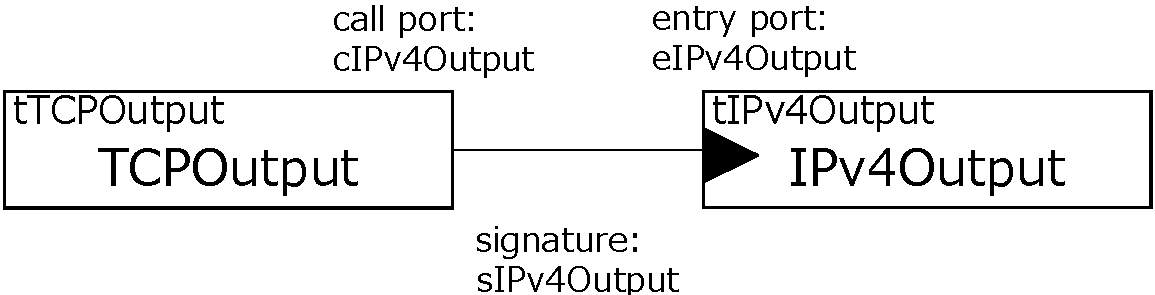
\includegraphics[width=8.0cm,clip]{figure/ComponentDiagram.pdf}
    \caption{Component diagram}
    \label{fig:ComponentDiagram}
\end{figure}

\subsubsection{Component model}

Fig. \ref{fig:ComponentDiagram} shows a component diagram.
{\it Cells}, which are instance of components in TECS, consist of {\it entry} ports, {\it call} ports, attributes, and internal variables.
An {\it entry} port is an interface that provides functions to other {\it cells}, whereas a {\it call} port is an interface that enables the use of other {\it cells}' functions.
Each {\it cell} has one or more {\it entry} ports and {\it call} ports.
{\it Cell} functions are implemented in C.

The type of {\it entry}/{\it call} port is defined by a {\it signature}, which is a set of functions that defines the interface definition of the {\it cell}.
The {\it cell's} {\it call} port can be connected to the {\it entry} port of another {\it cell} by the same {\it signature}.
Note that {\it celltype} defines one or more {\it call}/{\it entry} ports, attributes, and internal variables of a {\it cell}.

\subsubsection{Component description}

In TECS, components are described using component description language (CDL).
CDL can be divided into three categories: {\it signature}, {\it celltype}, and build description.
These components are described as follows.

\begin{description}
    \item[{\bf Signature Description}]\mbox{}\\
        The {\it signature} defines a {\it cell} interface.
        The {\it signature} name follows the keyword {\it signature} and takes the prefix ``s''--for instance, sIPv4Output (Fig. \ref{src:signature}).
        To clarify the function of an interface, specifiers such as [in], [out], and [inout] are used in TECS to represent the input, output, and input/output, respectively.
        Similarly, [size\_is({\it len})] represents an array of size {\it len}.
\begin{figure}[t]
\centering
\begin{lstlisting}
signature sIPv4Output {
  T_IN4_ADDR getIPv4Address(void);
  ER         getOffset([inout]T_OFF_BUF *offset);
  ER         setHeader([inout,size_is(size)]
                        int8_t *outputp,
                        [in]int32_t size,
                        [in]T_IN4_ADDR dstaddr,
                        [in]T_IN4_ADDR srcaddr);
    /* Omit: other functions */
};
\end{lstlisting}
\caption{Signature description}
\label{src:signature}
\end{figure}
    \item[{\bf Celltype Description}]\mbox{}\\
        The {\it celltype} defines the {\it entry} ports, {\it call} ports, attributes, and variables.
        A {\it celltype} name with the prefix ``t'' follows the keyword {\it celltype}, e.g., tIPv4Output (Fig. \ref{src:celltype}).
        To define {\it entry} ports, a {\it signature}, e.g., sIPv4Output, and an {\it entry} port name, e.g., eIPv4Output, follow the keyword {\it entry}.
        {\it Call} ports are defined similarly.
        Attributes and variables follow the keywords {\it attr} and {\it var}, respectively.
\begin{figure}[t]
\centering
\begin{lstlisting}
celltype tIPv4Output {
    /* Entry port */
    entry sIPv4Output eOutput;

    /* Call port */
    call sEthernetOutput cEthernetOutput;
    /* Omit: other call ports */

    attr {  /* Attribute */
        uint16_t fragInit = 0;
    };
    var {   /* Variable */
        uint16_t fragId = fragInit;
    };
};
\end{lstlisting}
\caption{Celltype description}
\label{src:celltype}
\end{figure}
    \item[{\bf Build Description}]\mbox{}\\
        The build description is used to instantiate and connect {\it cell}s.
        Fig. \ref{src:build} shows an example of a build description.
        A {\it celltype} name and {\it cell} name, e.g., tIPv4Output and IPv4Output, respectively, follow the keyword {\it cell}.
        A {\it call} port, {\it cell}'s name, and an {\it entry} port are described in that order to compose {\it cell}s,
        In Fig. \ref{src:build}, {\it entry} port eIPv4Output in {\it cell} IPv4Output is connected to {\it call} port cIPv4Output in {\it cell} TCPOutput.
        {\it C\_EXP} can be used to call macros defined in C files.

\begin{figure}[t]
\centering
\begin{lstlisting}
cell tIPv4Output IPv4Output {
    /* Omit: other build description */
    
    fragInit = 0; /* Attribute */
};
cell tTCPOutput TCPOutput {
    cIPv4Output = IPv4Output.eOutput;
    /* Omit: other build description */
};
\end{lstlisting}
\caption{Build description}
\label{src:build}
\end{figure}

\end{description}

\section{Design and Implementation}
\label{sec:Design and Implementation}

This section describes the design and implementation of the proposed TINET+TECS framework.
The proposed framework is a component-based TCP/IP protocol stack for embedded systems: in other words, a componentized TINET using TECS.
In this section, a new TECS functionality--the dynamic connection method--and the TECS adapter to support legacy codes are described via a use case of the proposed framework.

\subsection{TINET+TECS}
TINET+TECS, the proposed componentized TCP/IP protocol stack, comprises a number of some TECS components.
This section describes the components of the TINET+TECS framework with the aid of component diagrams.
% In addition, TECS functionalities applied to the proposed system such as {\it send}/{\it receive} specifier and adapter are explained.

\subsubsection{Components of a protocol stack}

The components of a TINET+TECS protocol stack are shown in Fig. \ref{fig:ComponentProtocolStack}.
Note that some small particle components, such as a kernel object, data queues, and semaphores, are omitted to simplify the component diagram.
In TINET+TECS, the components are divided for each protocol, and functionalities such as input and output functions are defined as respective components.
By using such small grain components, software visibility is improved.

\begin{figure}[t]
    \centering
    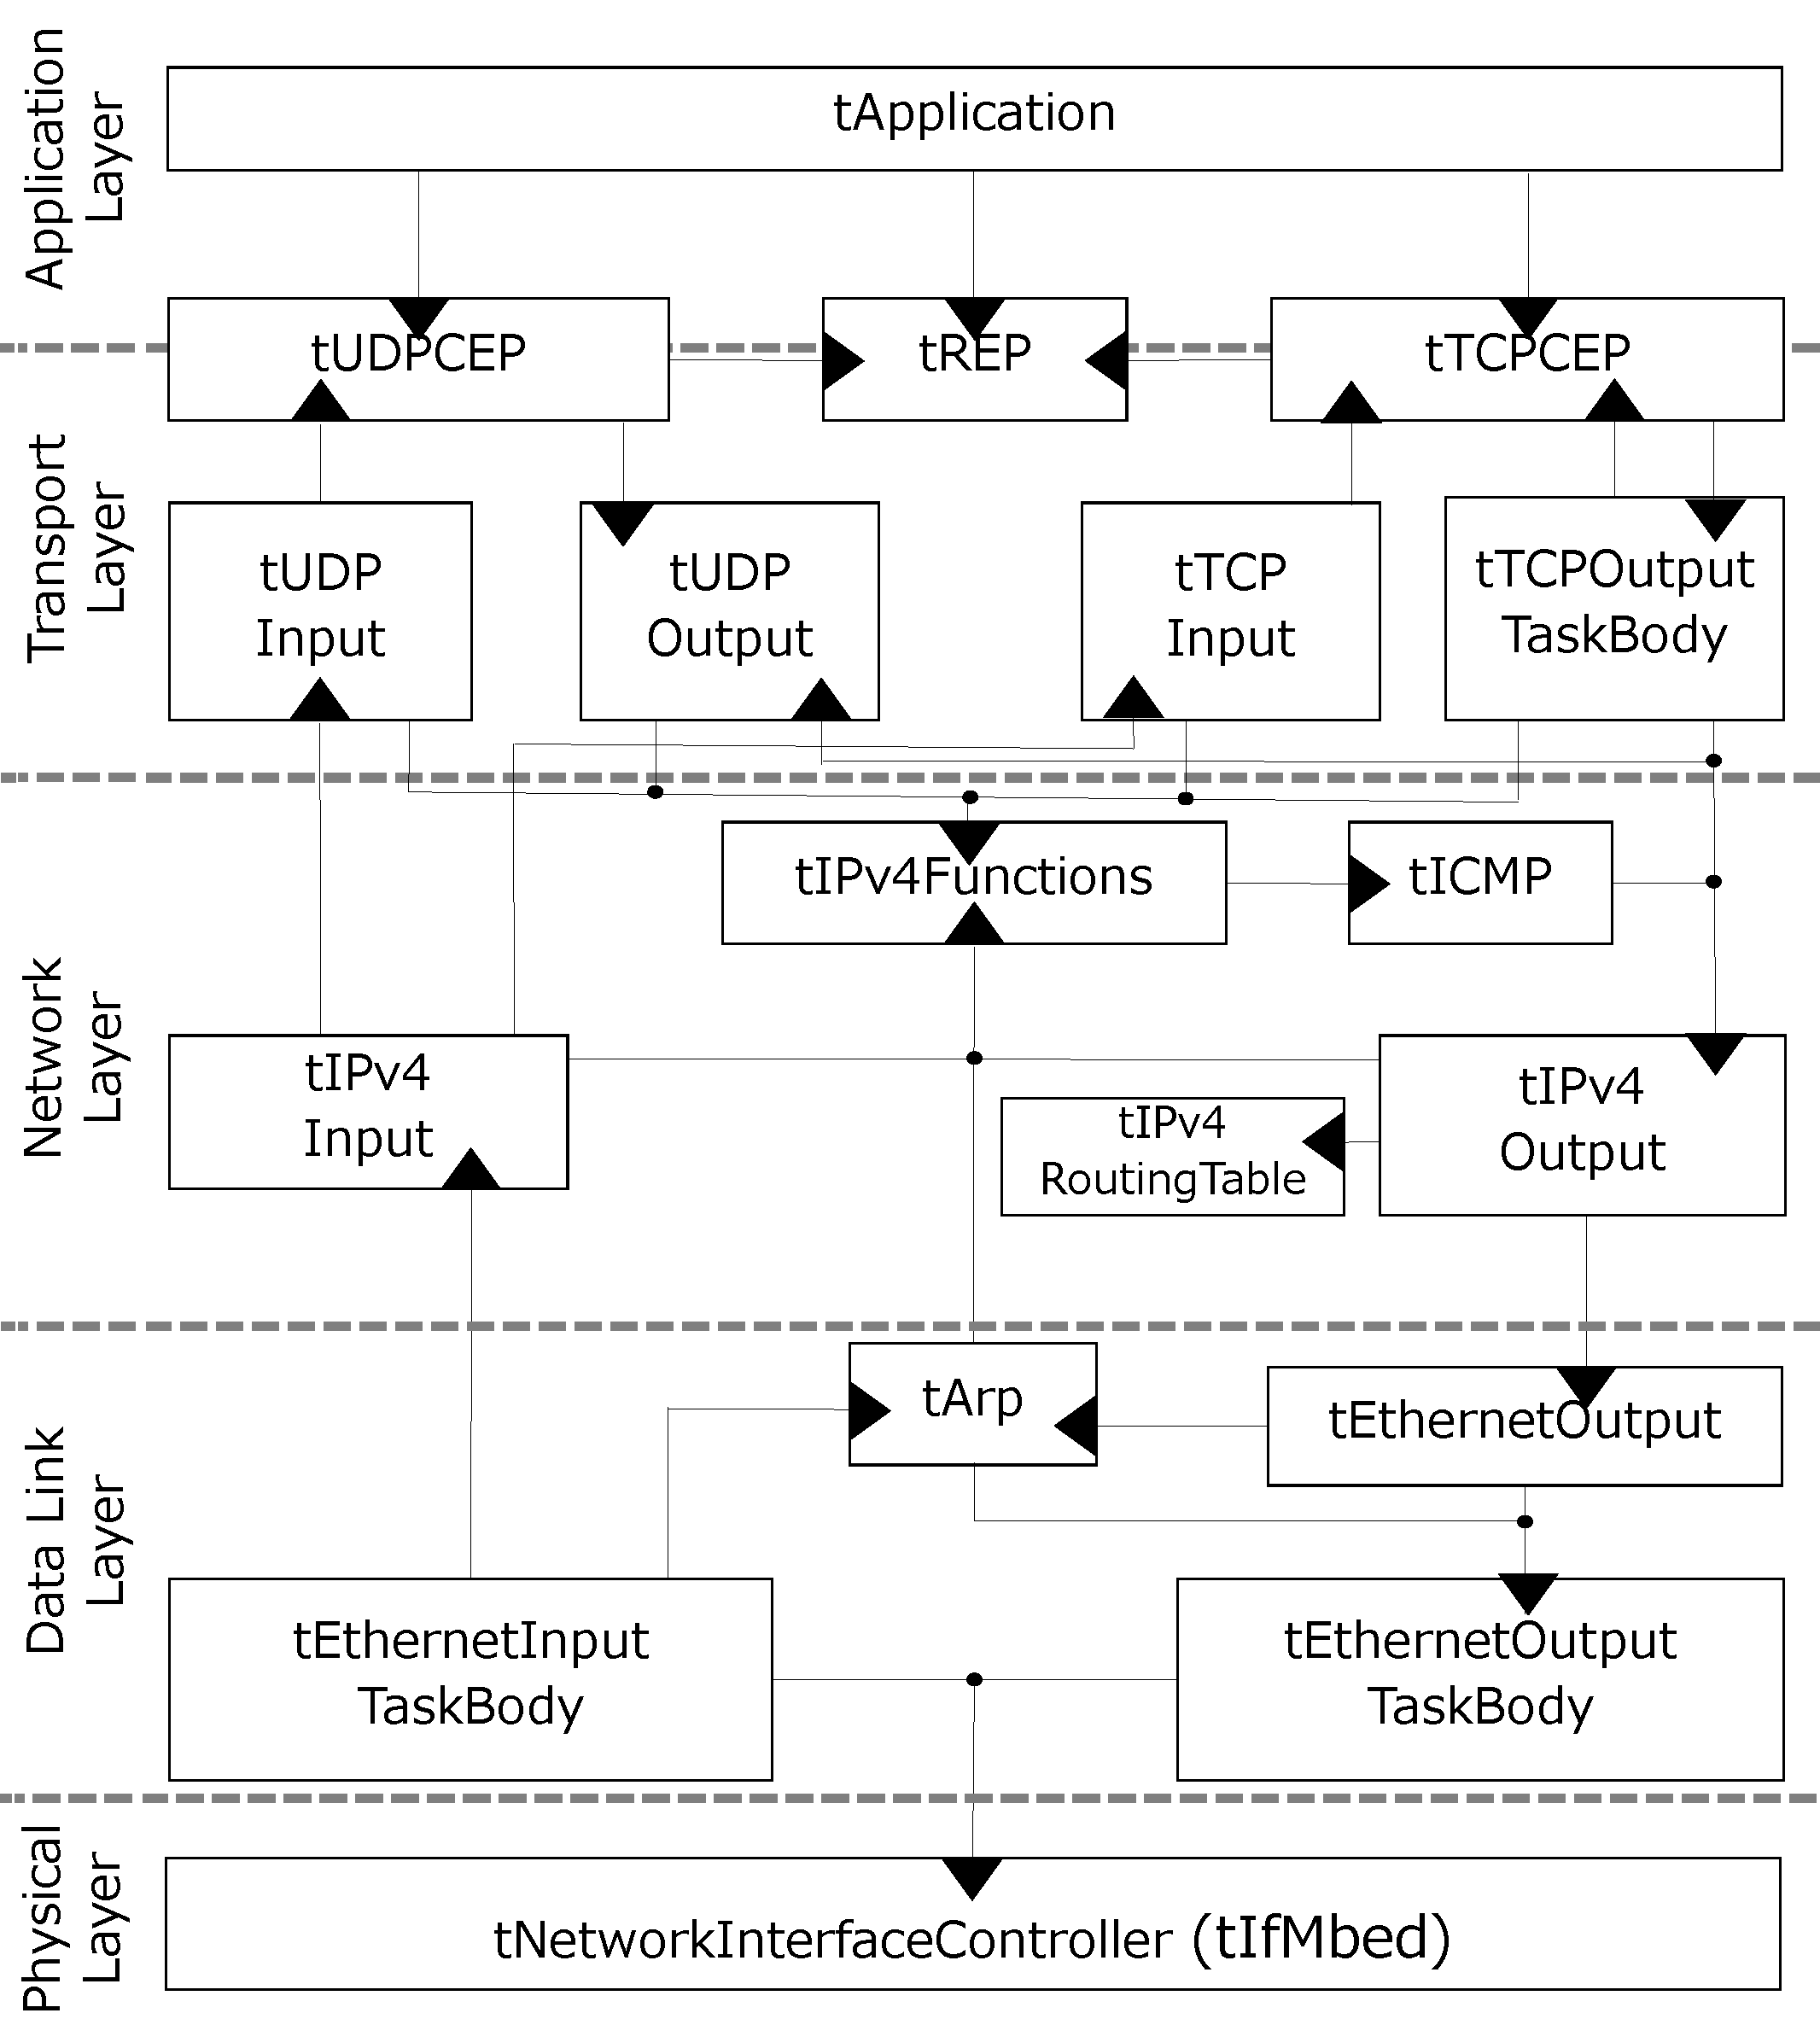
\includegraphics[width=8.0cm,clip]{figure/ComponentProtocolStack.pdf}
    \caption{Component diagram of a protocol stack}
    \label{fig:ComponentProtocolStack}
\end{figure}

The components of each protocol are described in the following.\\

{\bf Application layer:}
An application in TINET+TECS is implemented as a component such as tApplication.
Software with TINET uses ITRON TCP/IP API \cite{url:ITRON_TCP/IP_API_Spec} such as {\it tcp\_snd\_dat} and {\it tcp\_rcv\_dat}.
In TINET+TECS, the application component calls TECS functions such as {\it cTCPAPI\_sendData} and {\it cTCPAPI\_receiveData}.
Moreover, in TINET+TECS supporting a TECS adapter (\ref{sec:TECS Adapter}), an existing application with TINET can run on the TINET+TECS framework without transporting, and therefore, software can be developed either using existing methods or as TECS components.

{\bf Transport layer:}
tTCPCEP (tUDPCEP) and tREP are, respectively, CEP and REP components TCP (UDP).
For example, a server program supporting multiple clients can be developed by preparing multiple tTCPCEP components.
tTCPInput (tUDPInput) and tTCPOutput (tUDPOutput) are components for performing, respectively, receiving and sending processing in the transport layer.

{\bf Network layer:}
tIPv4Input and tIPv4Output are components that perform, respectively, the receiving and sending processing in the network layer.
The tIPv4Functions component performs functions such as checksum, the tICMP component is for implementing the Internet Control Message Protocol (ICMP), and the tIPv4RoutingTable component operates a routing table.

{\bf Data link layer:}
tEthernetInputTaskBody and tEthernetOutputTaskBody (tEthernetOutput) are components for performing, respectively, receiving and sending processing in the data link layer.
The tArp component is used for the Address Resolution Protocol (ARP).

{\bf Physical layer:}
The tNetworkInterfaceContoroller component implements a network device driver.
Software can be run on other devices by replacing the component because only the component depends on the target device.\\

To utilize the protocol stack in the same manner in the original TINET, communication object components such as tTCPCEP, tUDPCEP, and tREP are defined as an interface between TINET+TECS and an application.
The communication object component corresponds to a CEP or REP of the original TINET.
Application developers can utilize the TINET+TECS functionalities by generating and combining as many components as necessary.

The protocol stack of TINET+TECS supports the coexistence of multiple protocols.
Though its use of IPv6 and Point-to-Point Protocol (PPP) components, TINET+TECS can make IPv4 and IPv6 coexist and support PPP without modification of component implementation.

\subsubsection{Memory allocator component} 

The original TINET eliminates dynamic memory control to meet the severe memory restrictions of embedded systems.
A memory area for sending/receiving data in the protocol stack is allocated and released within a predetermined area.
The memory allocator component allows for elimination of dynamic memory control in TINET+TECS by providing a requested memory area from the statically allocated memory area.

The memory allocator component connects to as many tFixedSizeMemoryPool as required, as shown in Fig. \ref{fig:tMemoryAllocator}.
tFixedSizeMemoryPool is a componentized kernel object of TOPPERS/ASP3 for allocating and release memory areas of a requested size. 
tFixedSizeMemoryPool components of various sizes are prepared, and an appropriate memory area can be allocated according to the used data size.
On the other hand, all components that need to allocate or deallocate memory, e.g., tTCPInput and tEthernetOutput, connect to the memory allocator component.

In addition, TINET+TECS utilizes the TECS {\it send/receive} specifier to minimize the memory copy frequency, which is a functionality supported by TINET.

\begin{figure}[t]
    \centering
    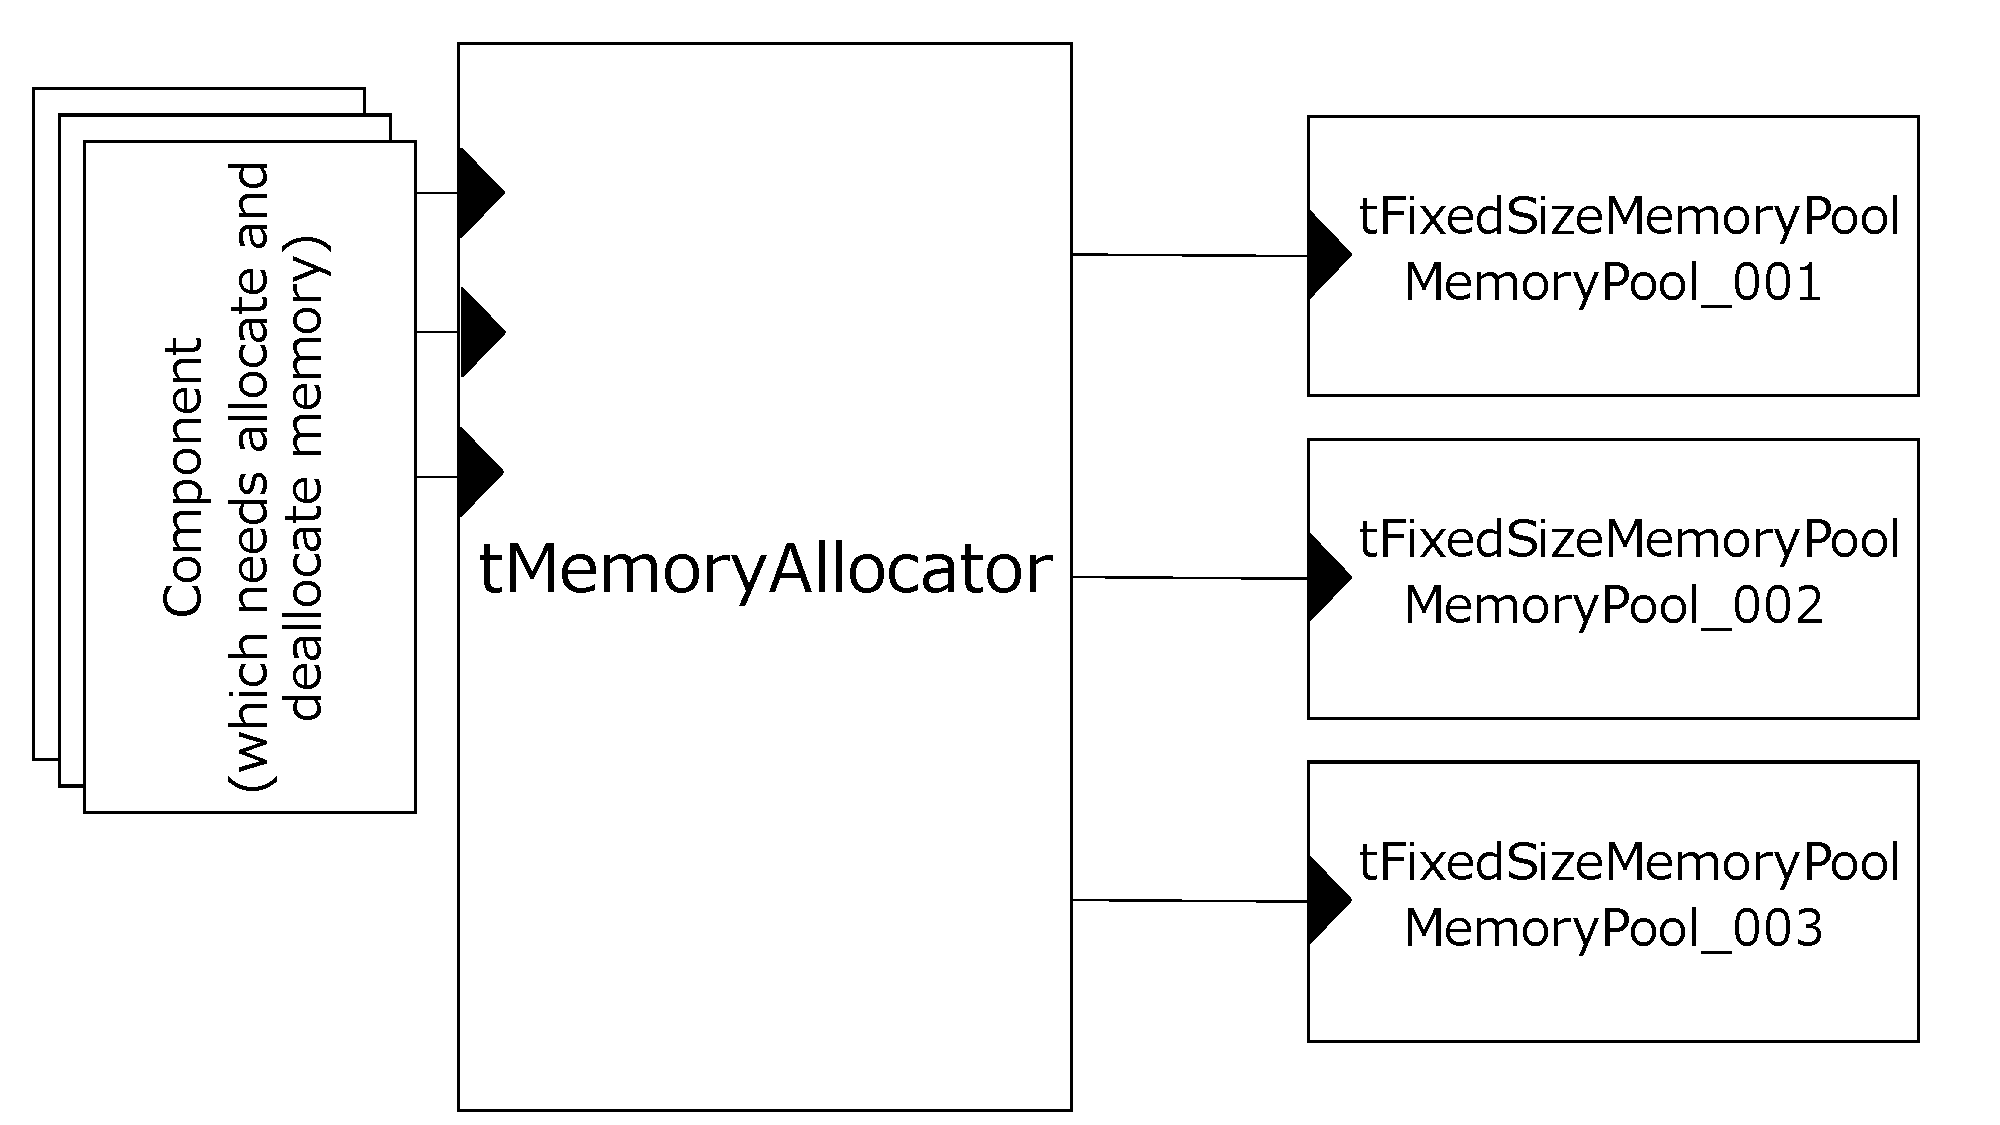
\includegraphics[width=8.0cm,clip]{figure/tMemoryAllocator.pdf}
    \caption{Component diagram of tMemoryAllocator}
    \label{fig:tMemoryAllocator}
\end{figure}

\begin{figure}[t]
    \centering
    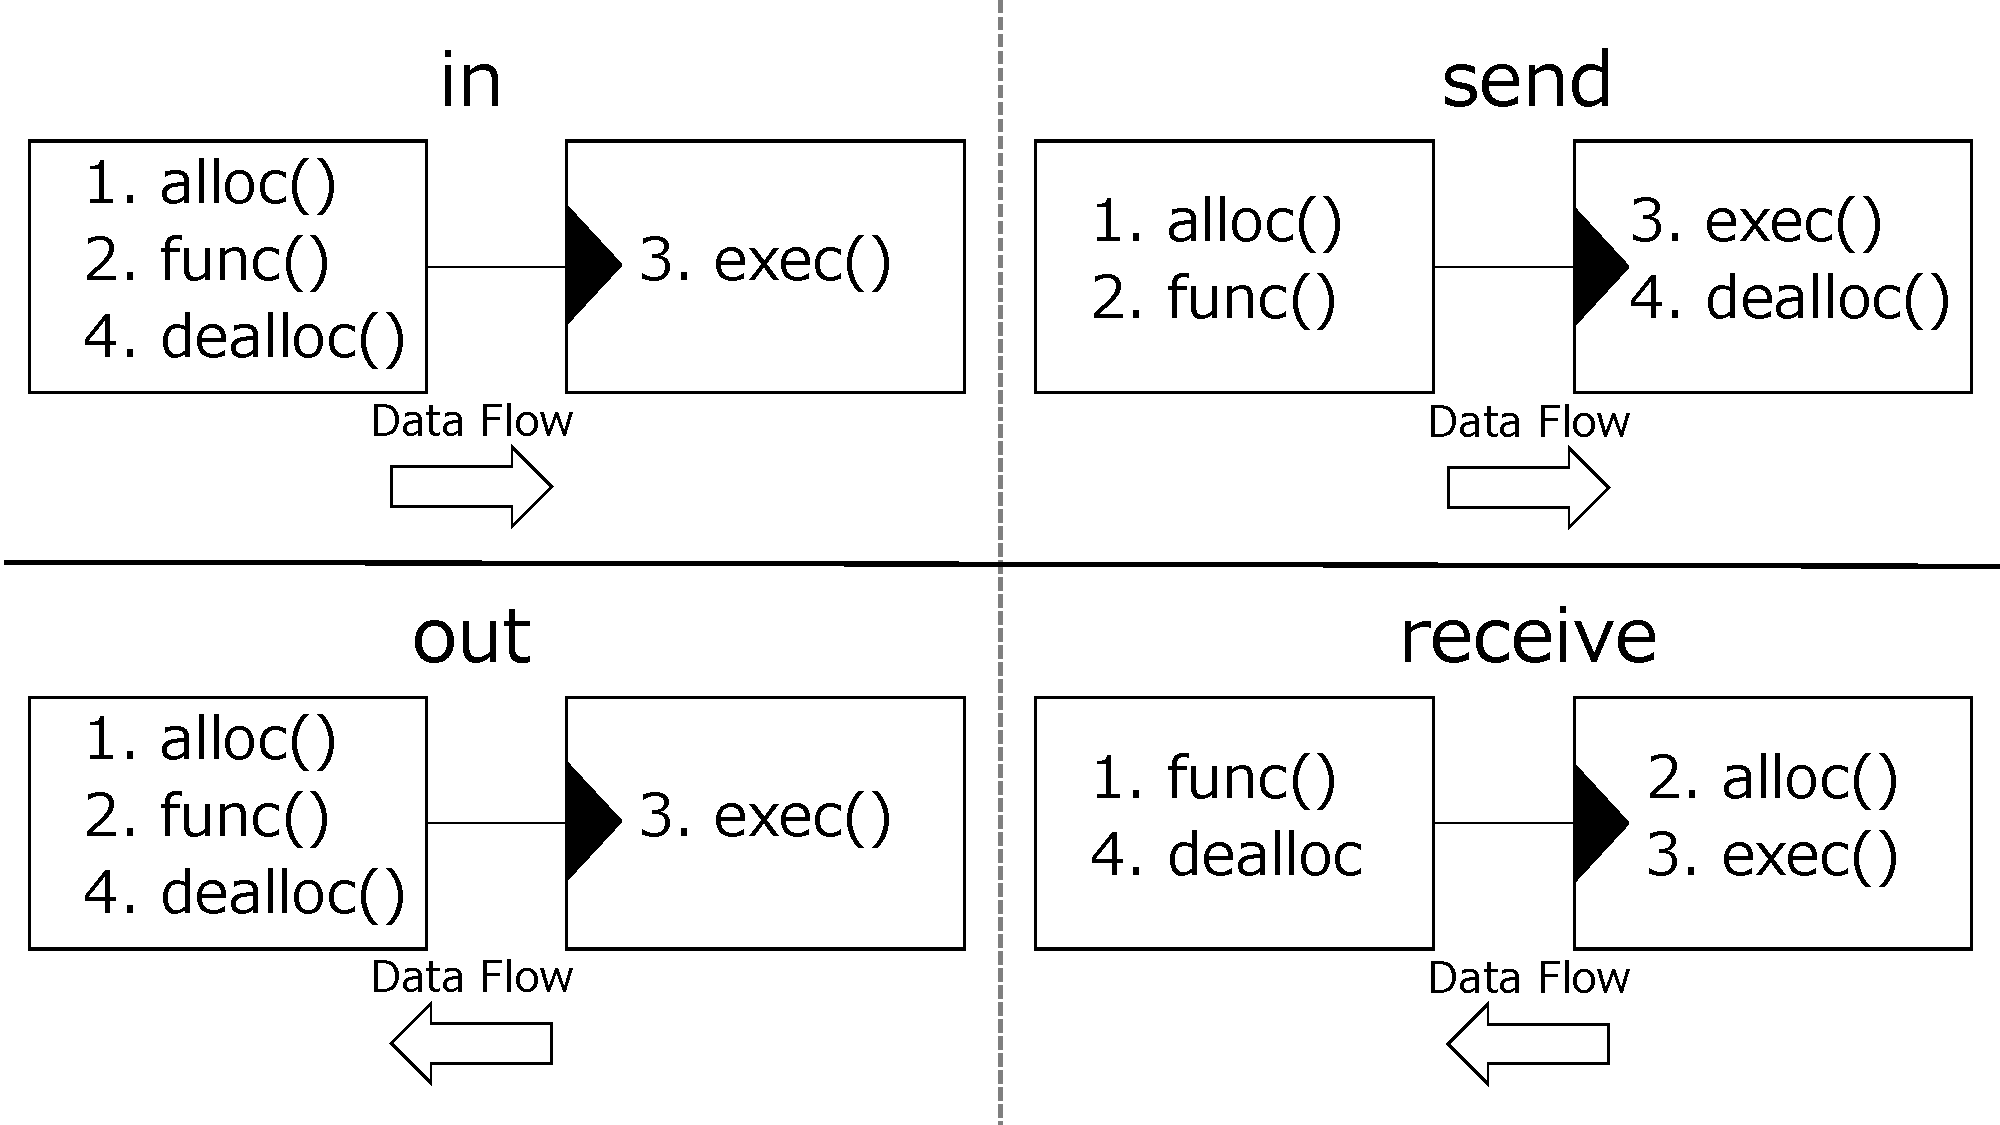
\includegraphics[width=8.0cm,clip]{figure/SendReceive.pdf}
    \caption{Differences between in/out and send/receive}
    \label{fig:SendReceive}
\end{figure}

{\bf Send/receive specifiers:}
TECS supports {\it send}/{\it receive} interface specifiers \cite{par:RPC}.
TINET+TECS uses {\it send} and {\it receive} specifiers instead of {\it in} and {\it out} to reduce the number of copies:

\begin{itemize}
\item {\it in} is a specifier for input arguments.
A callee side uses the memory of arguments with {\it in} when executing the callee function.
When the processing returns to the caller side, the caller can reuse and deallocate the memory.

\item {\it send} is another specifier for transferring data to a callee from a caller such as {\it in}.
The difference between {\it in} and {\it send} is whether the data memory is deallocated in the caller or callee, as shown in Fig. \ref{fig:SendReceive}.
In the case of the {\it in} specifier, both allocating and deallocating of the data memory are performed in the caller.
By contrast, in the case of {\it send}, the caller allocates the data memory and the callee deallocates it.

\item {\it out} is a specifier for output arguments through which a callee writes data in the memory allocated by a caller while the caller receives the data.

\item {\it receive} is another specifier for a caller receiving data from a callee such as {\it out}.
The difference between {\it out} and {\it receive} lies in whether the data memory is allocated in the caller or callee, as shown in Fig. \ref{fig:SendReceive}.
In the case of {\it out}, the callee writes data in the memory allocated by a caller, whereas in the {\it receive} case, the callee allocates the data memory.
Deallocating of the memory is performed in the caller in both cases.
\end{itemize}

As shown in Fig. \ref{src:SendReceive}, data sending and receiving arguments such as {\it outputp} and {\it inputp} are defined using, respectively, the {\it send/receive} specifier in the signature description.

\begin{figure}[t]
\centering
\begin{lstlisting}
signature sNicDriver {
  void start(
    [send(sNetworkAlloc),size_is(size)]
        int8_t *outputp,
    [in]int32_t size,
    [in]uint8_t align);
  void read(
    [receive(sNetworkAlloc),size_is(*size)]
        int8_t **inputp,
    [out]int32_t *size,
    [in]uint8_t align);
    /* Omit: other functions */
};
\end{lstlisting}
\caption{Signature description of the nic driver (An example of send/receive)}
\label{src:SendReceive}
\end{figure}

% \subsubsection{Network timer component}


\subsection{Dynamic connection in TECS}
\label{sec:DynamicConnection}

\begin{figure}[t]
    \centering
    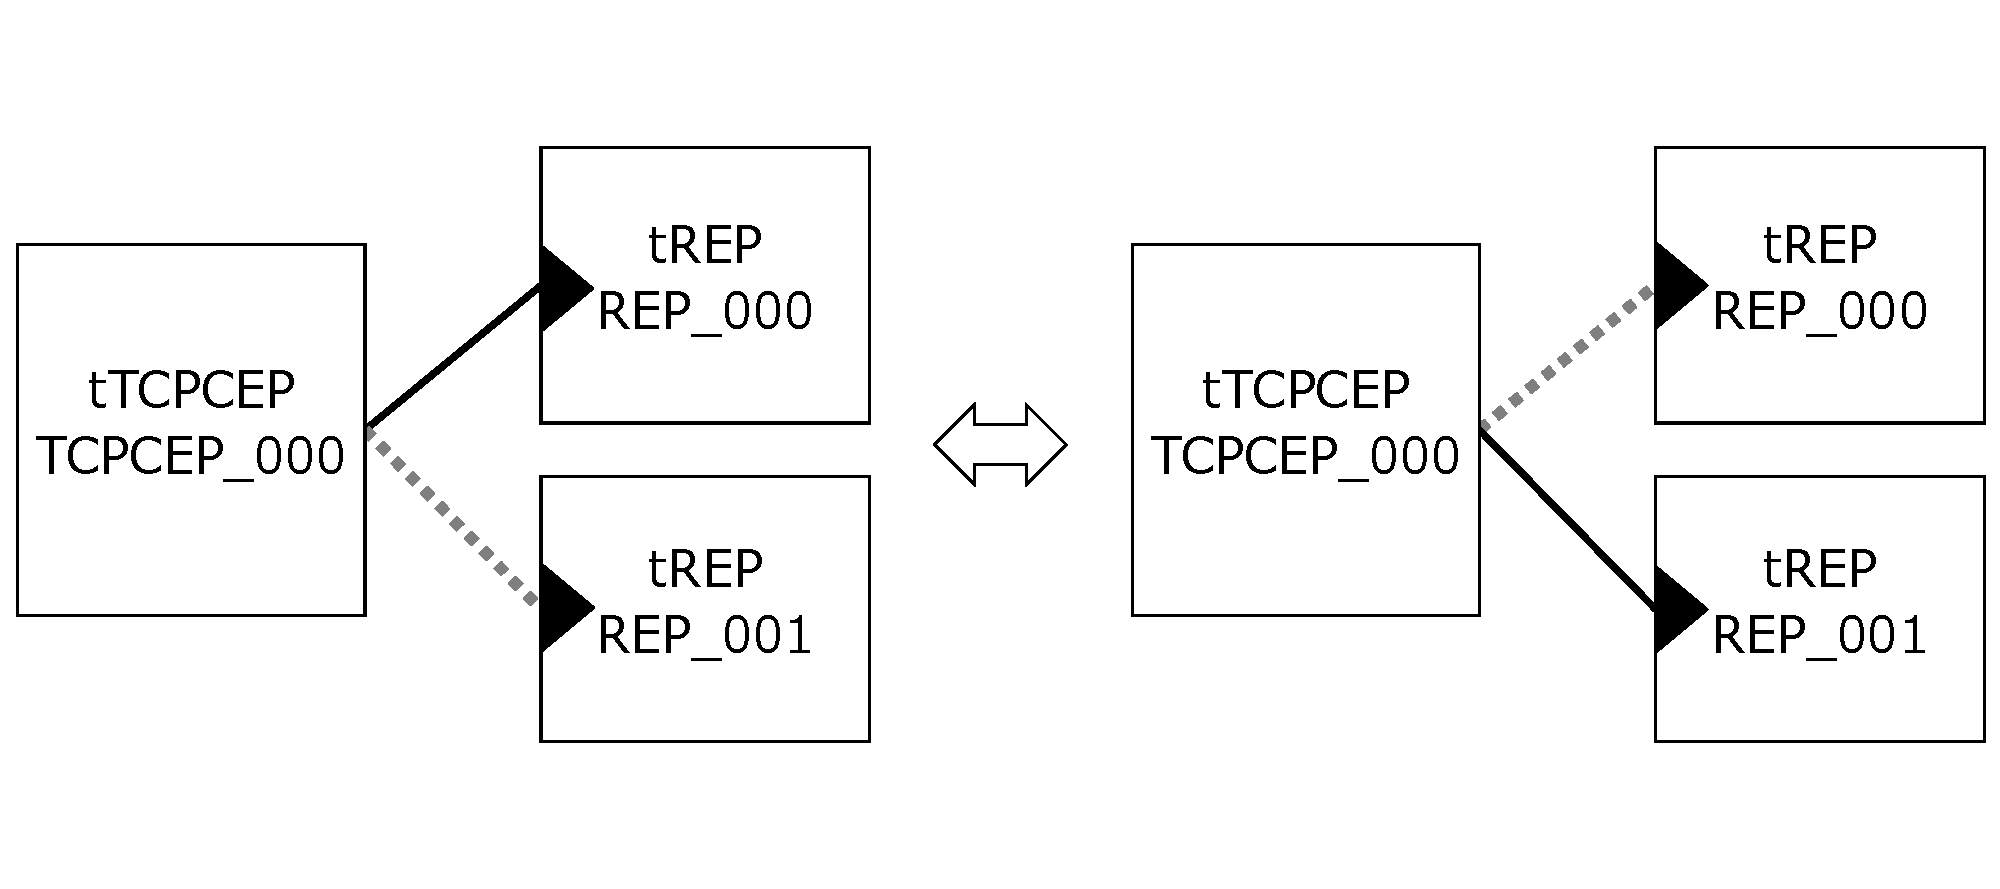
\includegraphics[width=8.0cm,clip]{figure/DynamicConnection.pdf}
    \caption{Dynamic connection}
    \label{fig:DynamicConnection}
\end{figure}

TECS supports dynamic connection, a method for switching the binding of components at runtime (Fig. \ref{fig:DynamicConnection}) as a new functionality.
Note that all components are statically generated in TECS, which can optimize the overhead of componentization because components are statically configured.
Dynamically generating components causes a good deal of memory consumption, which is a serious problem for embedded systems with strict memory constraints.
The proposed framework can take advantage of the componentization in TINET while satisfying the memory constraint because components are statically generated and dynamically connected in TECS.

TINET+TECS utilizes dynamic connection to switch between CEP and REP components, as shown in Fig. \ref{fig:DynamicConnectionUseCase}.
In a server application, CEP is associated with REP in the state of waiting for connection request from clients\footnote{ITRON TCP/IP API Specification \cite{url:ITRON_TCP/IP_API_Spec}\\tcp\_acp\_cep(ID cepid, ID repid, T\_IPV4EP *p\_dstaddr, TMO tmout).}.
For example, when processing with the HTTP protocol, CEP passively opens with an REP of port number 80.

\begin{figure}[t]
    \centering
    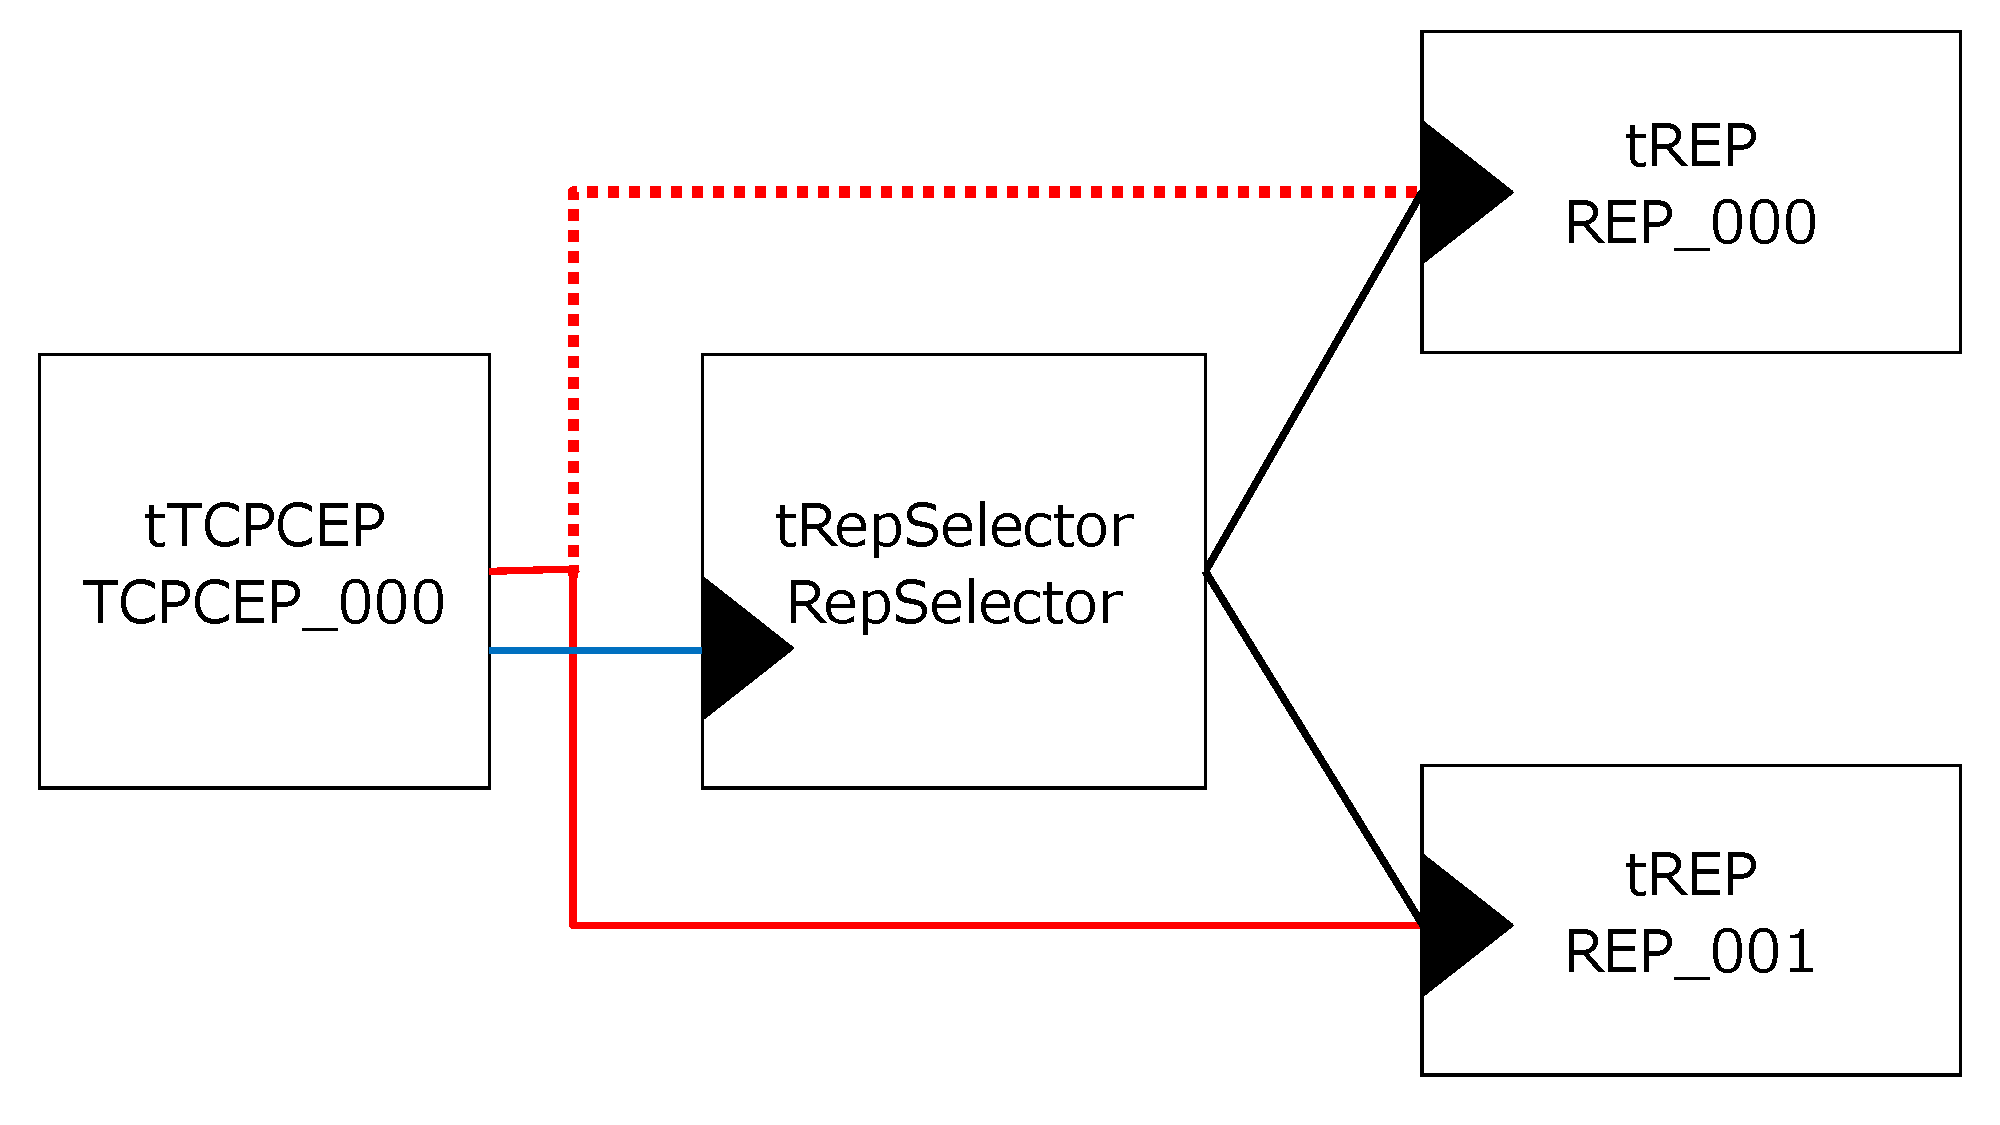
\includegraphics[width=8.0cm,clip]{figure/DynamicConnectionUseCase.pdf}
    \caption{Dynamic connection between CEP and REP}
    \label{fig:DynamicConnectionUseCase}
\end{figure}

To utilize dynamic connectivity, a selector should be defined.
A selector connects all components that can be dynamically connected under a common descriptor that serves as an identifier to access each component \cite{par:optimization}.
The cREP ports form a call port array connecting to connecting to all tREP cells (Line 9 in Fig. \ref{src:DynamicCDLcode}).
{\it [ref\_desc]} is used to identify call ports referring to descriptors. 
In the case shown in Fig. \ref{fig:DynamicConnectionUseCase}, the tRepSelector cell connects all tREP cells.

A CEP component has two call ports: the cRepSelector port, which connects to the eRepSelector port of tRepSelector cell, and the cREP4 port, which connects to either of the tREP cells (Lines 13--15 in Fig. \ref{src:DynamicCDLcode}).
The cREP port is defined using {\it [dynamic]} to identify the call port used to dynamically switch the components.
The call port with the {\it [dynamic]} specifier is not optimized and is allocated in RAM using a plug-in.

\begin{figure}[t]
\centering
\begin{lstlisting}
signature sRepSelector {
    void  getRep([out]Descriptor(sREP4) *desc,
                 [in]int_t i);
};

celltype tRepSelector {
    entry sRepSelector eRepSelector;
    [ref_desc]
        call sREP4 cREP[NUM_REP];
};

celltype tTCPCEP {
    call sRepSelector cRepSelector;
    [dynamic]
        call sREP4 cREP;
    /* Omit: other call/entry ports */
    /* Omit: attributes and variables */
};
\end{lstlisting}
\caption{Signature and celltype description for dynamic connection}
\label{src:DynamicCDLcode}
\end{figure}

Fig. \ref{src:DynamicCcode} shows a sample code of dynamic connection.
The eAPI\_accept function is the function wrapping {\it tcp\_acp\_cep} under TECS, which is set as the state waiting for connection request.
Dynamic connection in the function is performed as shown in Fig. \ref{src:DynamicCcode}.
First, the descriptor of REP to be joined is obtained (Line 3 in Fig. \ref{src:DynamicCcode}).
The first argument, {\it \&desc}, is a variable used to store the descriptor information, whereas the second argument, {\it repid}, is the index of tREP cells.
Next, the descriptor is set (Line 5 in Fig. \ref{src:DynamicCcode}), and the cREP port combines the tREP cell specified by the descriptor, enabling the tCEP cell to call the function of the tREP cell to be joined (Line 7 in Fig. \ref{src:DynamicCcode}).

\begin{figure}[t]
\centering
\begin{lstlisting}
eAPI_accept (.., ..) {
    /* Get a descriptor of intended REP cell */
    cRepSelector_getRep(&desc, repid);
    /* Set the descriptor */
    cREP_set_descriptor(desc);
    /* Call the function of intended REP cell */
    cREP_getEndpoint();
}
\end{lstlisting}
\caption{Accept function (Dynamic connection example)}
\label{src:DynamicCcode}
\end{figure}

\subsection{TECS adapter}
\label{sec:TECS Adapter}

TECS supports {\it Adapter} functionality, which enables to calling a function in TECS from existing C codes.
The adapter is implemented between C codes and a TECS component and links a C function to a TECS function as shown in Fig. \ref{fig:TECS_Adapter}.
In TINET+TECS, when an application calls an API such as {\it tcp\_snd\_dat}, the adapter component calls a function of tTCPCEP such as {\it eAPI\_sendData}.
Note that {\it tcp\_snd\_dat} is defined under the name {\it eAPI\_sendData} in TINET+TECS.
The adapter wraps the APIs used in the existing applications into TECS functions, enabling software developers to utilize an existing TCP/IP application via the adapter.

\begin{figure}[t]
    \centering
    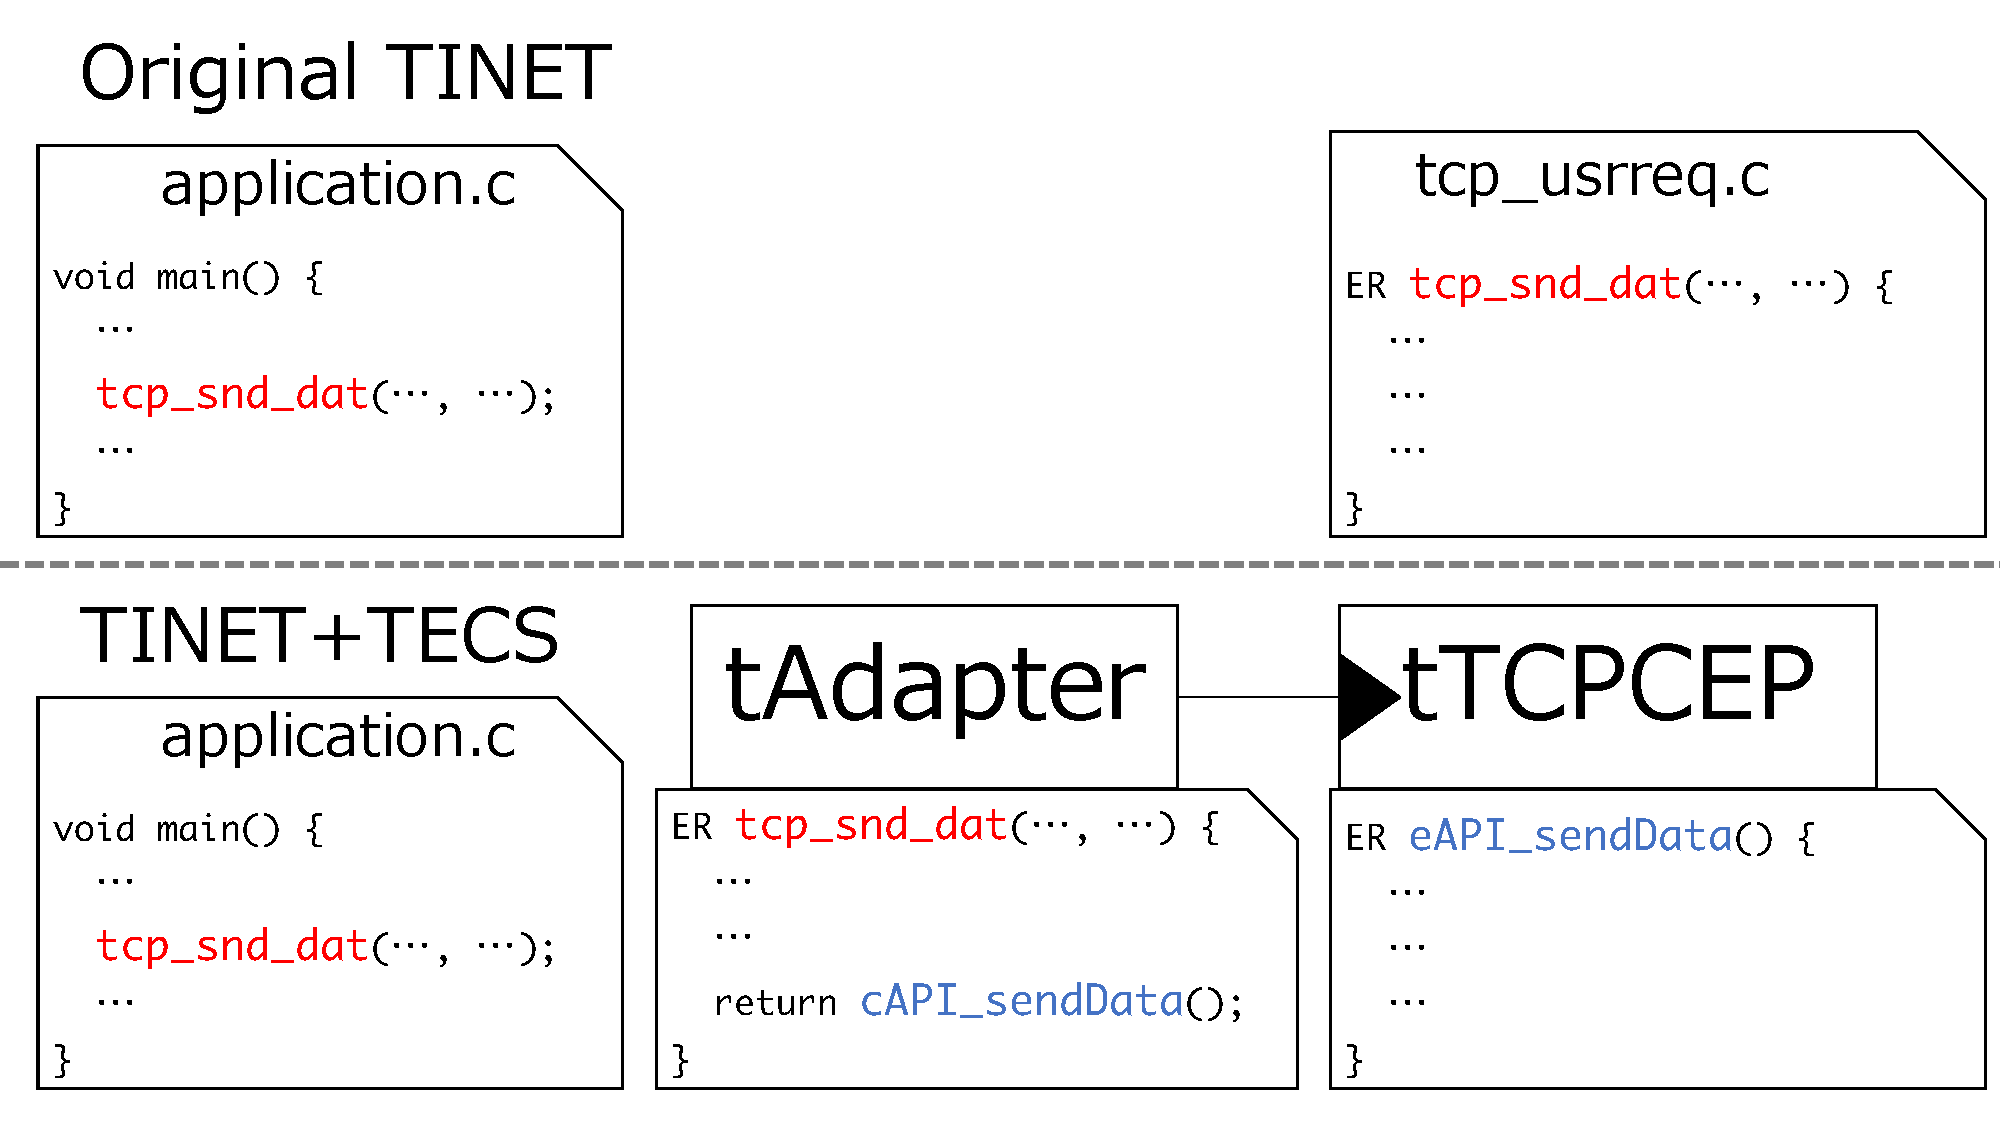
\includegraphics[width=8.0cm,clip]{figure/TECS_Adapter.pdf}
    \caption{TECS adapter}
    \label{fig:TECS_Adapter}
\end{figure}

\section{Evaluation}
\label{sec:Evaluation}

This section describes the experimental evaluation used to demonstrate the effectiveness of the proposed framework.

\subsection{Evaluation environment}

GR-PEACH was employed as the evaluation board.
Detailed specifications of the board are shown in TABLE \ref{tab:EvaluationBoardEnvironment}.
We also employ TINET 1.5.4 and the compiler arm-none-eabi--gcc 5.2
To pretest the system, we connected the board to a host PC via a LAN cable and evaluated the data transmission and reception.

\begin{table}[t]
    \centering
    \caption{Evaluation Board Environment}
    \begin{tabular}{l|l}
        \hline\hline
        Board           &   GR-PEACH                \\
        CPU             &   Cortex-A9 RZ/A1H 400MHz \\
        Flash ROM       &   8 MB                    \\
        RAM             &   10 MB                   \\
        LAN Controller  &   LAN8710A                \\
        \hline
    \end{tabular}
    \label{tab:EvaluationBoardEnvironment}
\end{table}

\subsection{Performance of TINET+TECS}

To demonstrate the low overhead of TINET+TECS, we compared its execution time and memory consumption with that of TINET, producing the comparison results shown in Fig. \ref{fig:EvaluationOfExecutionTime}.

The {\it tcp\_snd\_dat} and {\it tcp\_rcv\_dat} APIs were used in the evaluation to, respectively, send and receive TCP data.
For {\it tcp\_snd\_dat}, we measured the executing time starting from the API call through the application until the return of the processing result.
In TINET+TECS, this process is performed in the order tApplication, tTCPCEP, tTCPOutputTaskBody, tIPv4Output, tEthernetOutput, tArp, tEthernetOutputTaskBody, and tIfMbed, as shown in Fig. \ref{fig:ComponentProtocolStack}.
For {\it tcp\_rcv\_dat}, we measured the execution time from the data receipt in the LAN driver until data acquisition in the application.
In TINET+TECS, the process is performed in the order tIfMbed, tEthernetInputTaskBody, tIPv4Input, tTCPInput, tTCPCEP, and tApplication, as shown in Fig. \ref{fig:ComponentProtocolStack}.
The execution time of TINET+TECS is close to that of TINET, with an overhead of about 3 ms.
As the use of the {\it send/receive} specifier enables accessing of the buffer address without data copying, the componentization overhead does not affect the execution time.

\begin{figure}[t]
    \centering
    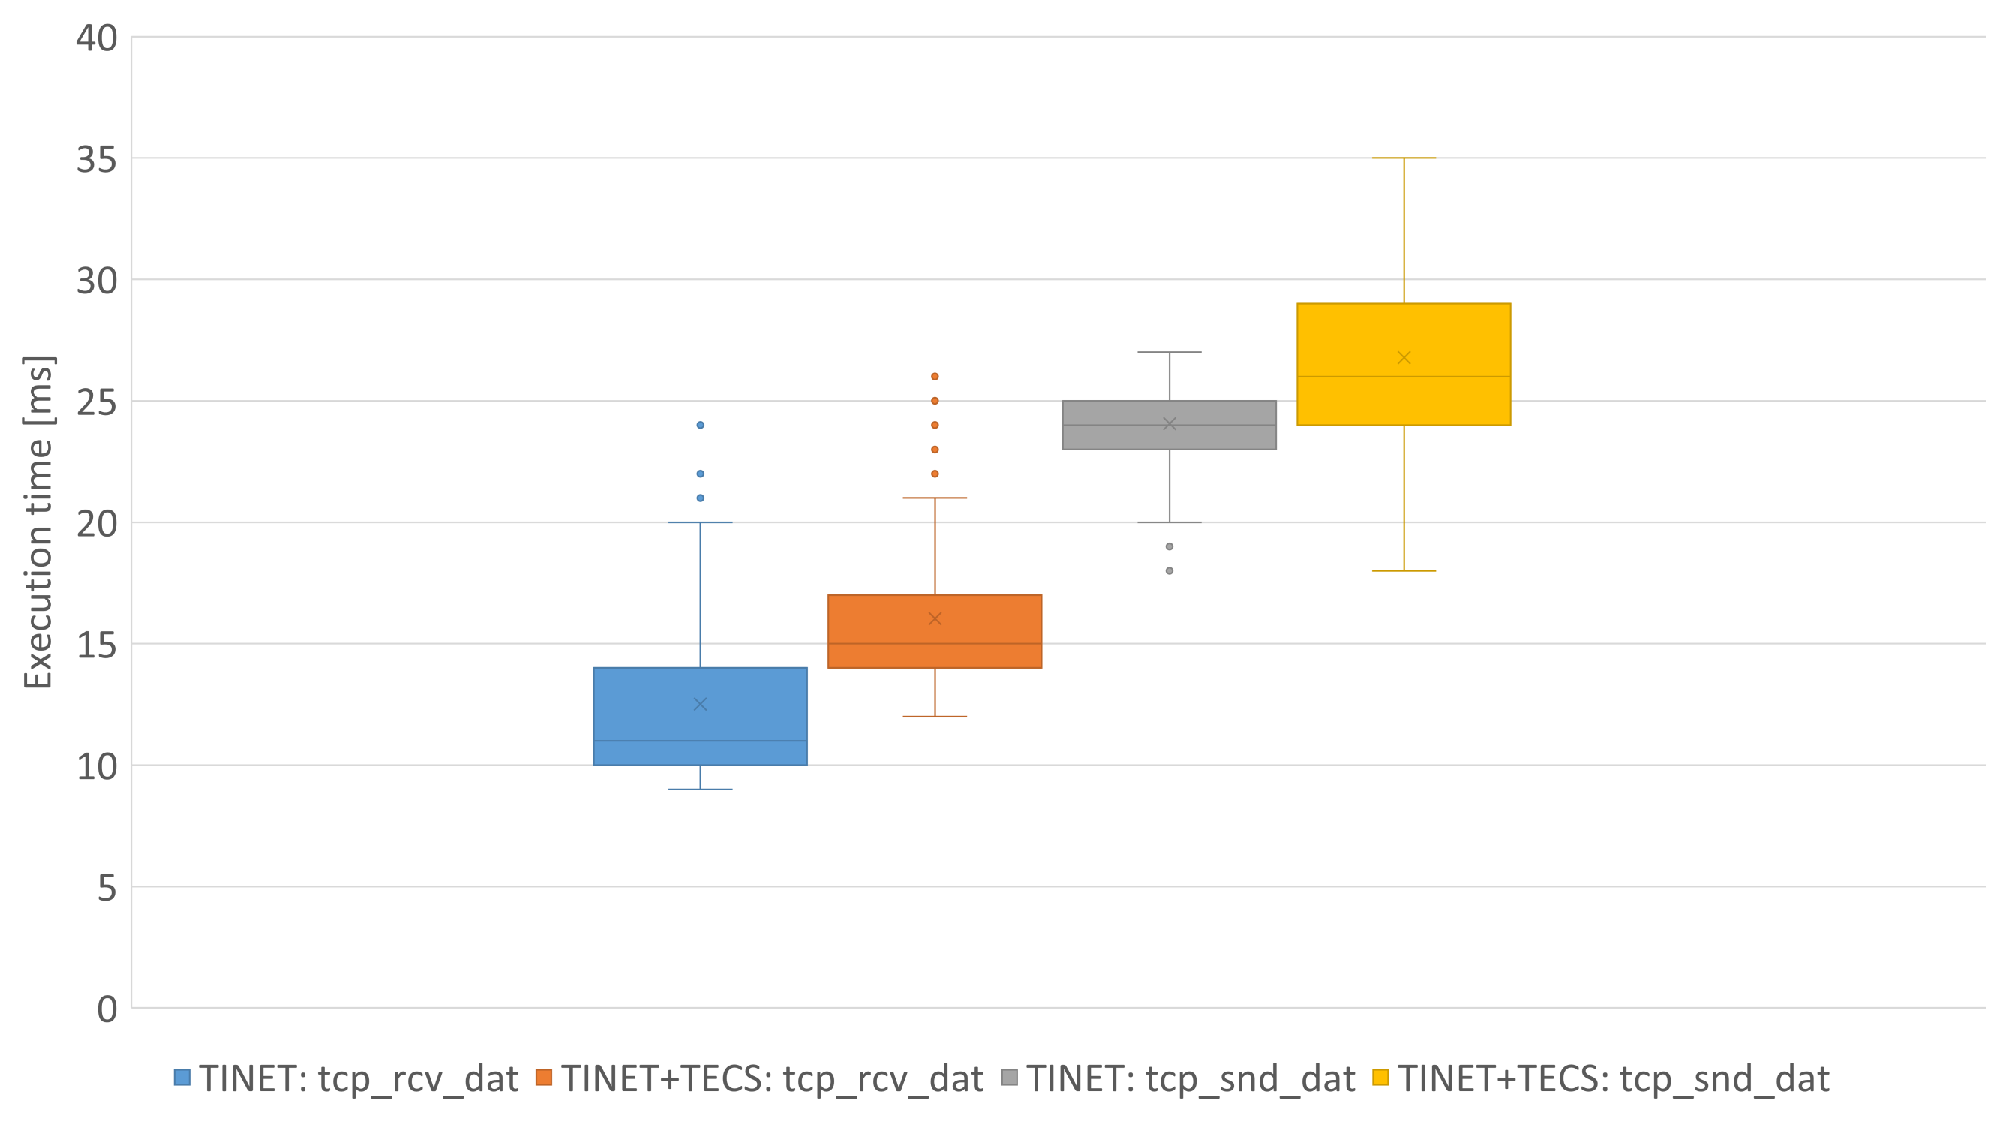
\includegraphics[width=8.0cm,clip]{figure/EvaluationOfExecutionTime.pdf}
    \caption{Execution times of TINET and TINET+TECS}
    \label{fig:EvaluationOfExecutionTime}
\end{figure}

The memory consumptions of TINET and TINET+TECS are compared in TABLE \ref{tab:EvaluationOfMemoryConsumption}.
The memory consumption of TINET+TECS is about 1\% higher than that of TINET, as the data and processes such as initialization of cells, descriptors, function tables, and skeleton functions needed to manage TECS components increase memory consumption.

\begin{table}[t]
    \centering
    \caption{Memory consumption of TINET and TINET+TECS}
    \begin{tabular}{c|r|r|r|r}
        \hline\hline
                    &   text       &  data    &   bss      &  total     \\ \hline
        TINET       &   183.94 KB  &  5.37 KB &  132.03 KB &  322.34 KB \\
        TINET+TECS  &   170.73 KB  &  5.37 KB &  149.13 KB &  325.23 KB \\
        \hline
        \multicolumn{5}{r}{Including the application and kernel objects}
    \end{tabular}
    \label{tab:EvaluationOfMemoryConsumption}
\end{table}

As shown in TABLE \ref{tab:EvaluationOfConfigurabilty}, the code lines for modification were measured to demonstrate the improved configurability.
This demonstrated the ability to change the composition of the protocol stack with a small workload, confirming that the proposed framework improves the configurability.

\begin{table}[t]
    \centering
    \caption{Modified code lines of CDL}
    \begin{tabular}{c|r|r|r}
        \hline\hline
                         &   Size       &   Size (- Default)  & CDL  \\ \hline
        Default          &   325.23 KB  &             0 KB    &  0 lines   \\
        I                &   305.40 KB  &       - 19.83 KB    & 18 lines    \\
        I + I\hspace{-.1em}I &   304.12 KB  &   - 21.10 KB    & 27 lines   \\
        I + I\hspace{-.1em}I + I\hspace{-.1em}I\hspace{-.1em}I & 303.45 KB & - 21.77 KB  & 32 lines \\
        \hline
        \multicolumn{4}{l}{I: Remove TCP}\\
        \multicolumn{4}{l}{I\hspace{-.1em}I: Remove ICMP}\\
        \multicolumn{4}{l}{I\hspace{-.1em}I\hspace{-.1em}I: Change network buffer (Remove memory pools)}
    \end{tabular}
    \label{tab:EvaluationOfConfigurability}
\end{table}


\subsection{Dynamic connection}

\begin{figure}[t]
    \centering
    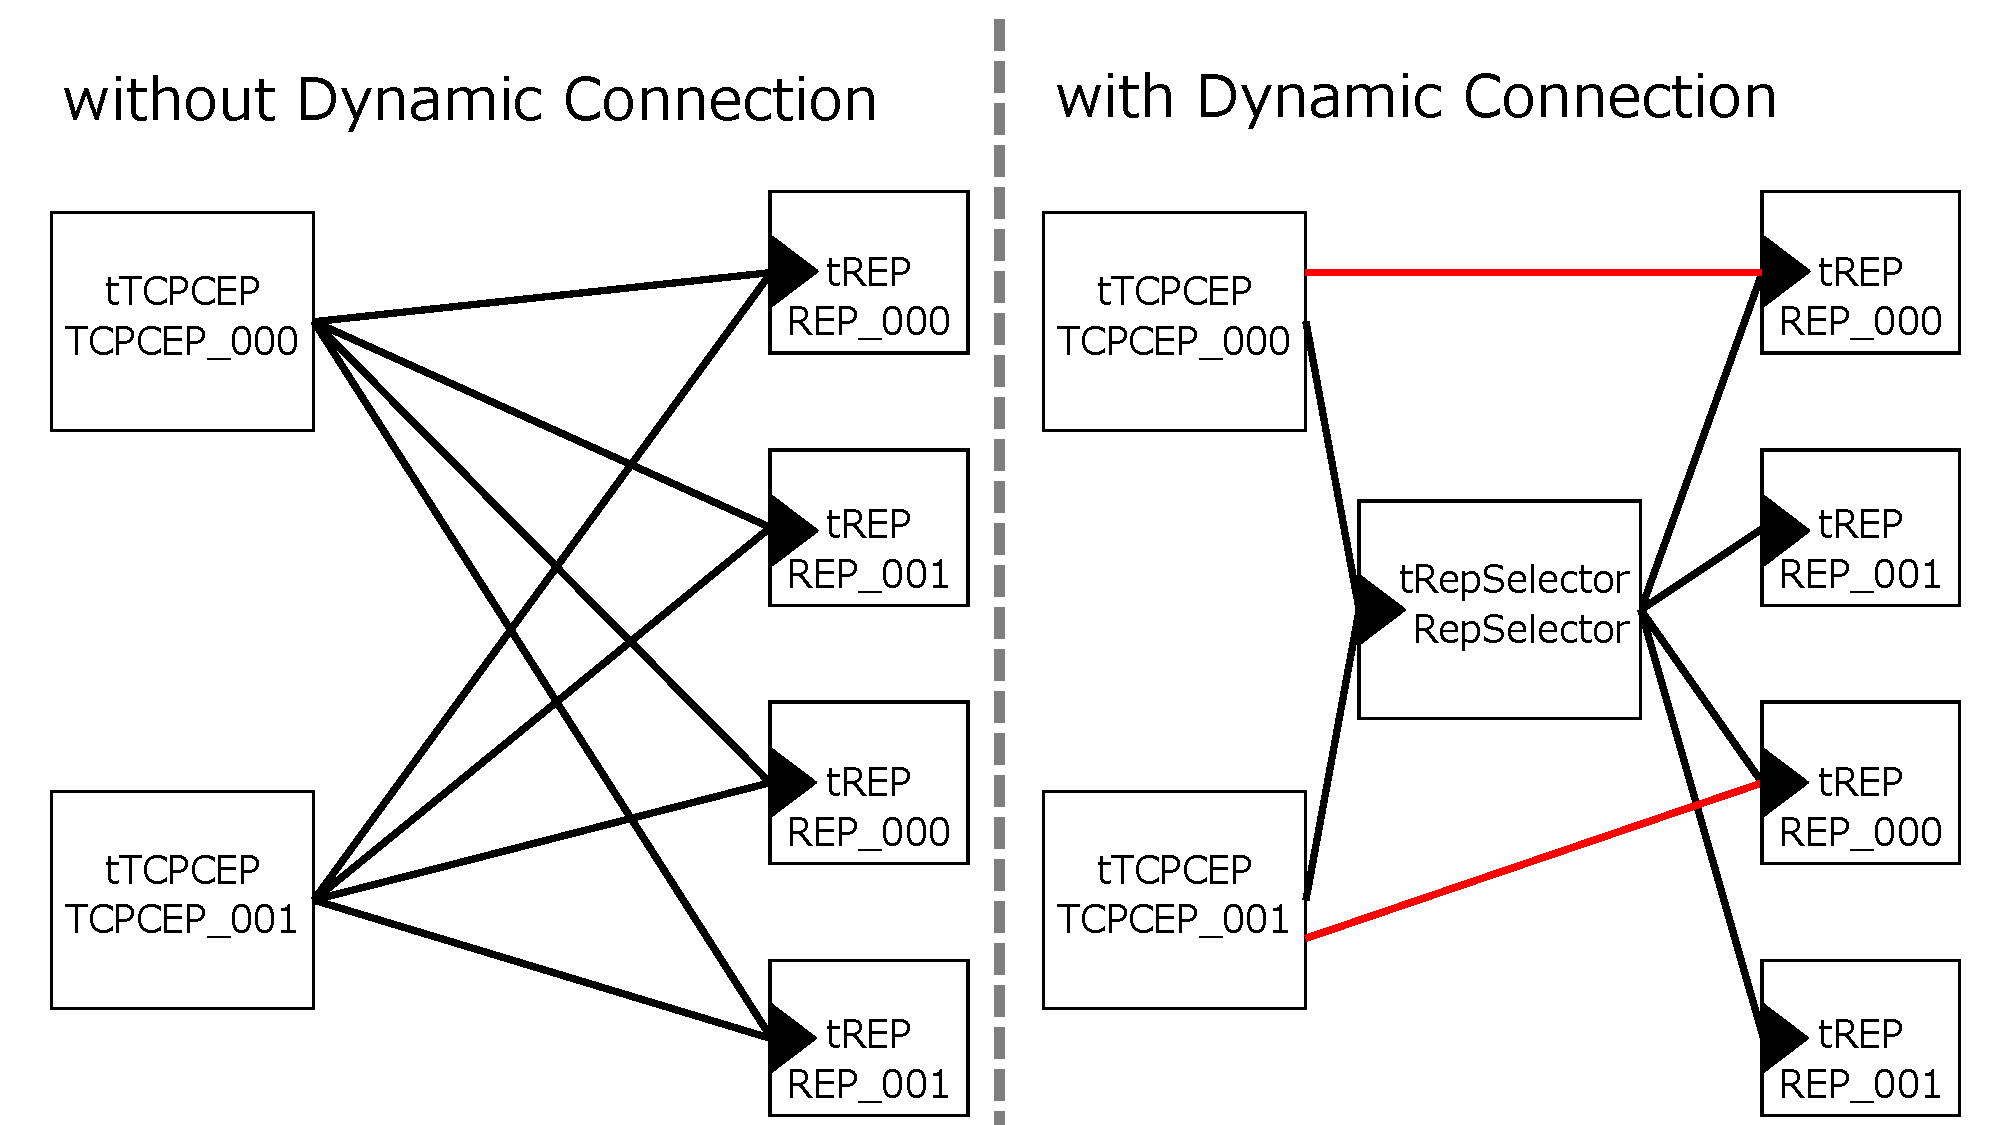
\includegraphics[width=8.0cm,clip]{figure/ComparisonOfDynamicConnection.pdf}
    \caption{Component diagrams for two cases (without/with dynamic connection)}
    \label{fig:ComparisonOfDynamicConnection}
\end{figure}

Memory consumption without and with TECS dynamic connection was then evaluated.
As shown in the left panel of Fig. \ref{fig:ComparisonOfDynamicConnection}, each CEP component should be statically connected to all REP components if dynamic connection is not used.
As the number of REPs increases, additional call ports of CEP are required, in turn increasing the consumption of memory. 
Dynamic connection reduces memory consumption because only one CEP-to-REP call port is required per CEP, as illustrated with red lines in the right panel of Fig. \ref{fig:ComparisonOfDynamicConnection}.
Even if the number of REPs increases, additional call ports can be joined through the selector, instead of the CEPs.

Memory consumption of without and with dynamic connection is shown in Fig. \ref{fig:EvaluationOfDynamicConnection}.
The dynamic connection case consumes the more RAM memory because, as mentioned in Section \ref{sec:DynamicConnection}, call ports with {\it [dynamic]} are not optimized and allocated in RAM areas.
However, the overall memory consumption is lower under the proposed framework.

\begin{figure}[t]
    \centering
    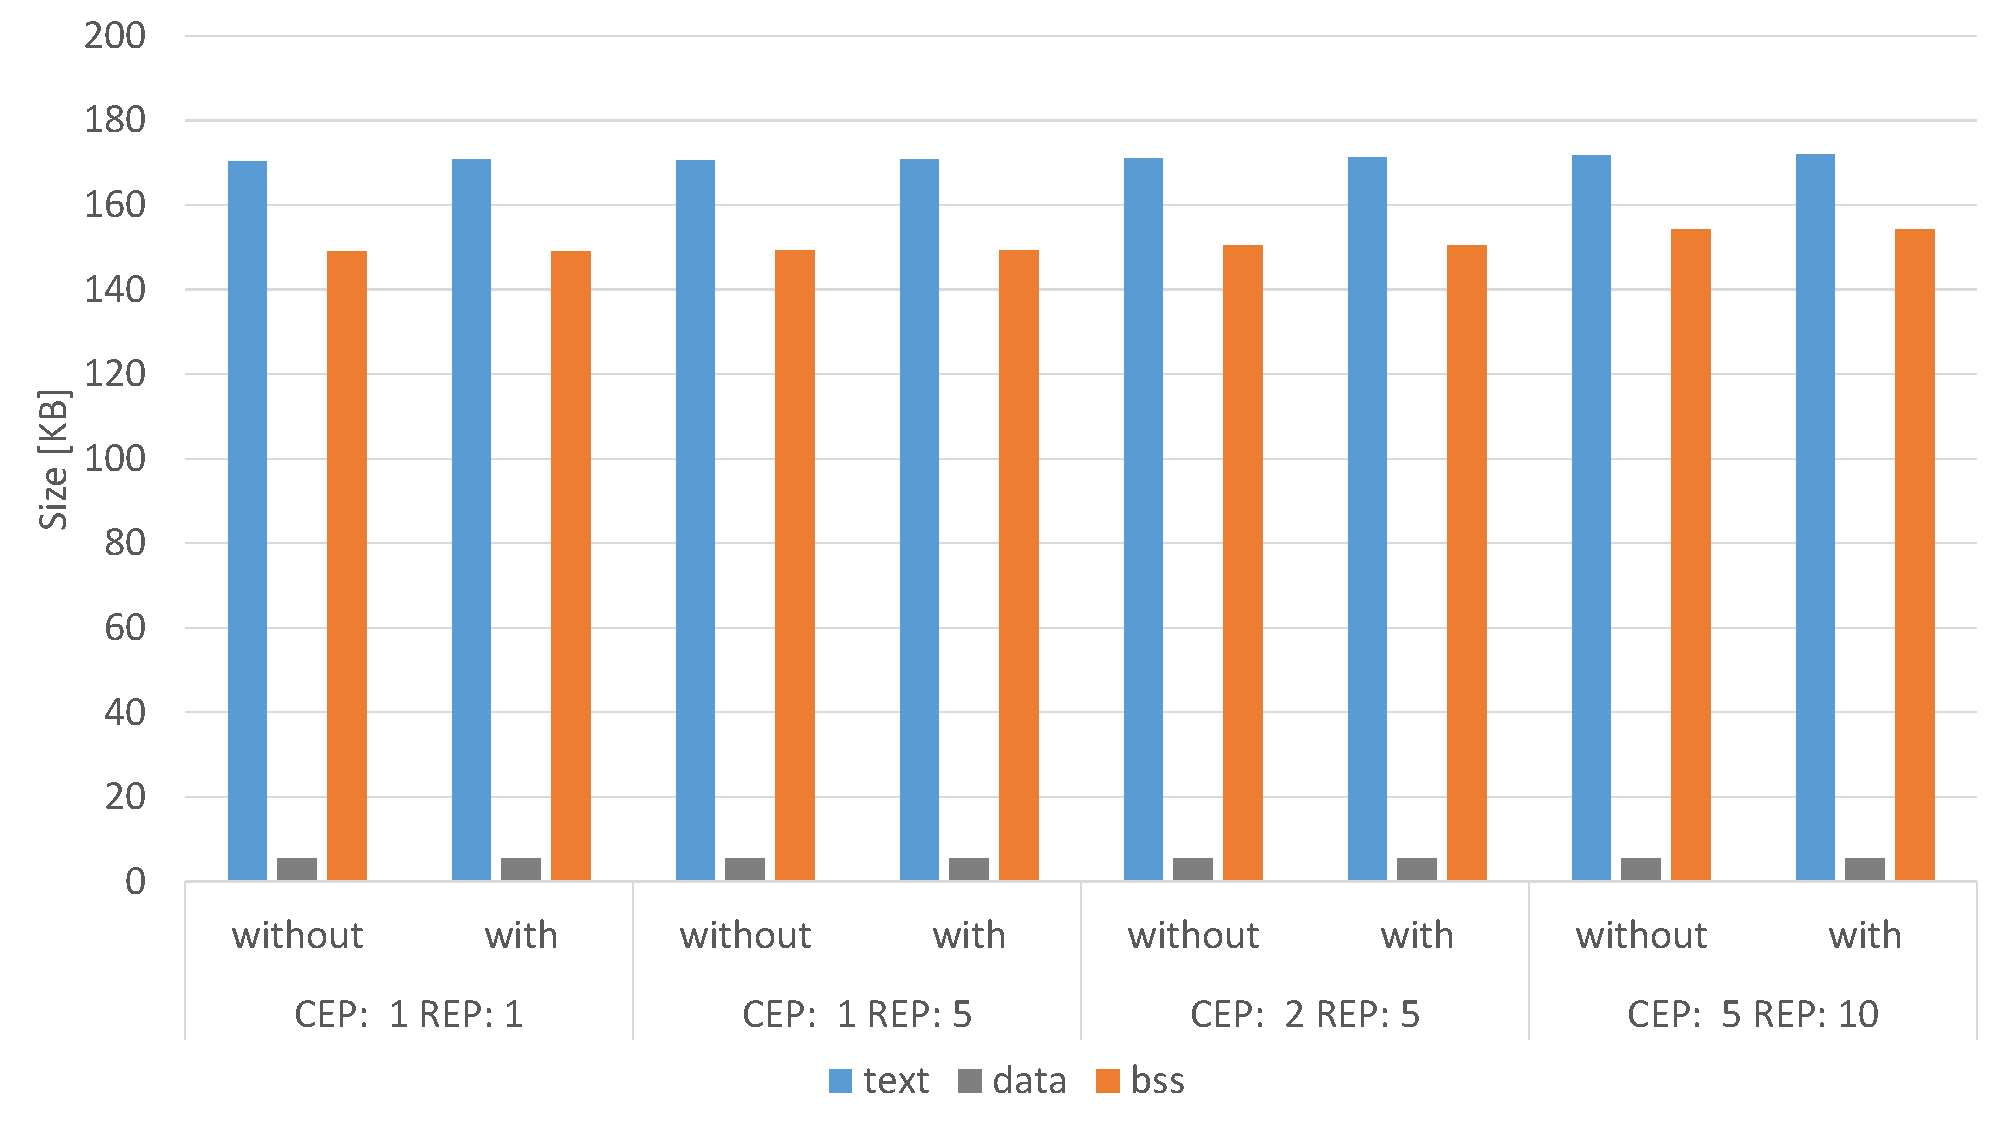
\includegraphics[width=8.0cm,clip]{figure/EvaluationOfDynamicConnection.pdf}
    \caption{Memory consumption in two cases (with/without dynamic connection)}
    \label{fig:EvaluationOfDynamicConnection}
\end{figure}

\begin{table}[t]
    \centering
    \caption{CDL code lines of without/with dynamic connection}
    \begin{tabular}{l|r|r|r}
        \hline\hline
                     &  without  &  with  &  Diff  \\ \hline
        CEP:1 REP:1  &  344 lines     &  347 lines  &  -3 lines   \\
        CEP:1 REP:5  &  369 lines     &  367 lines  &   2 lines   \\
        CEP:2 REP:5  &  387 lines     &  382 lines  &   5 lines   \\
        CEP:5 REP:10 &  485 lines     &  445 lines  &  40 lines   \\
        \hline
    \end{tabular}
    \label{tab:EvaluationOfConfigurabilityByDynamicConnection}
\end{table}

\begin{figure}[t]
 \centering
 \begin{lstlisting}
/* without Dynamic Connection */
cell tTCPCEP TCPCEP_000 {
    cREP[0] = REP_000.eREP;
    ..
    cREP[n] = REP_00n.eREP;
};
cell tTCPCEP TCPCEP_001 {
    cREP[0] = REP_000.eREP;
    ..
    cREP[n] = REP_00n.eREP;
};
..
cell tTCPCEP TCPCEP_00n {
    cREP[0] = REP_000.eREP;
    ..
    cREP[n] = REP_00n.eREP;
};
 \end{lstlisting}
 \centering
 \begin{lstlisting}
/* with Dynamic Connection */
cell tRepSelector RepSelector {
    cREP[0] = REP_000.eREP;
    ..
    cREP[n] = REP_00n.eREP;
};
cell tTCPCEP TCPCEP_000 {
    cRepSelector = RepSelector.eRepSelector;
};
cell tTCPCEP TCPCEP_001 {
    cRepSelector = RepSelector.eRepSelector;
};
..
cell tTCPCEP TCPCEP_00n {
    cRepSelector = RepSelector.eRepSelector;
};
 \end{lstlisting}
 \caption{Comparison of CDL descriptions between without/with dynamic connection}
 \label{src:ComparisonOfCDL}
\end{figure}

The comparison of CDL code lines of without and with dynamic connection is shown in TABLE \ref{tab:EvaluationOfConfigurabilityByDynamicConnection}, to demonstrate improved configurability by dynamic connection.
As the number of CEPs and REPs increases, the amount of CDL code lines to be added increases.
In the left panel of Fig. \ref{fig:ComparisonOfDynamicConnection}, each CEP connects all REPs as shown in the upper of Fig. \ref{src:ComparisonOfCDL}. 
In the right panel of Fig. \ref{fig:ComparisonOfDynamicConnection}, a CEP dynamically connects an REP, and only the selector connects all REPs as shown in the lower of Fig. \ref{src:ComparisonOfCDL}. 
It is effective for software that uses many ports because the difference spreads as the number of CEPs and REPs increases.

\subsection{Adapter overhead}

The API execution time when using an adapter such as {\it tcp\_snd\_dat/eAPI\_sendData} was used to analyze the overhead of the TECS adapter supporting existing applications.
As shown in Fig. \ref{fig:EvaluationOfAdapter}, the overhead of the TECS adapter is very small because the adapter only passes parameters from C codes to TECS components; thus, the TECS adapter overhead does not affect the system.

\begin{figure}[t]
    \centering
    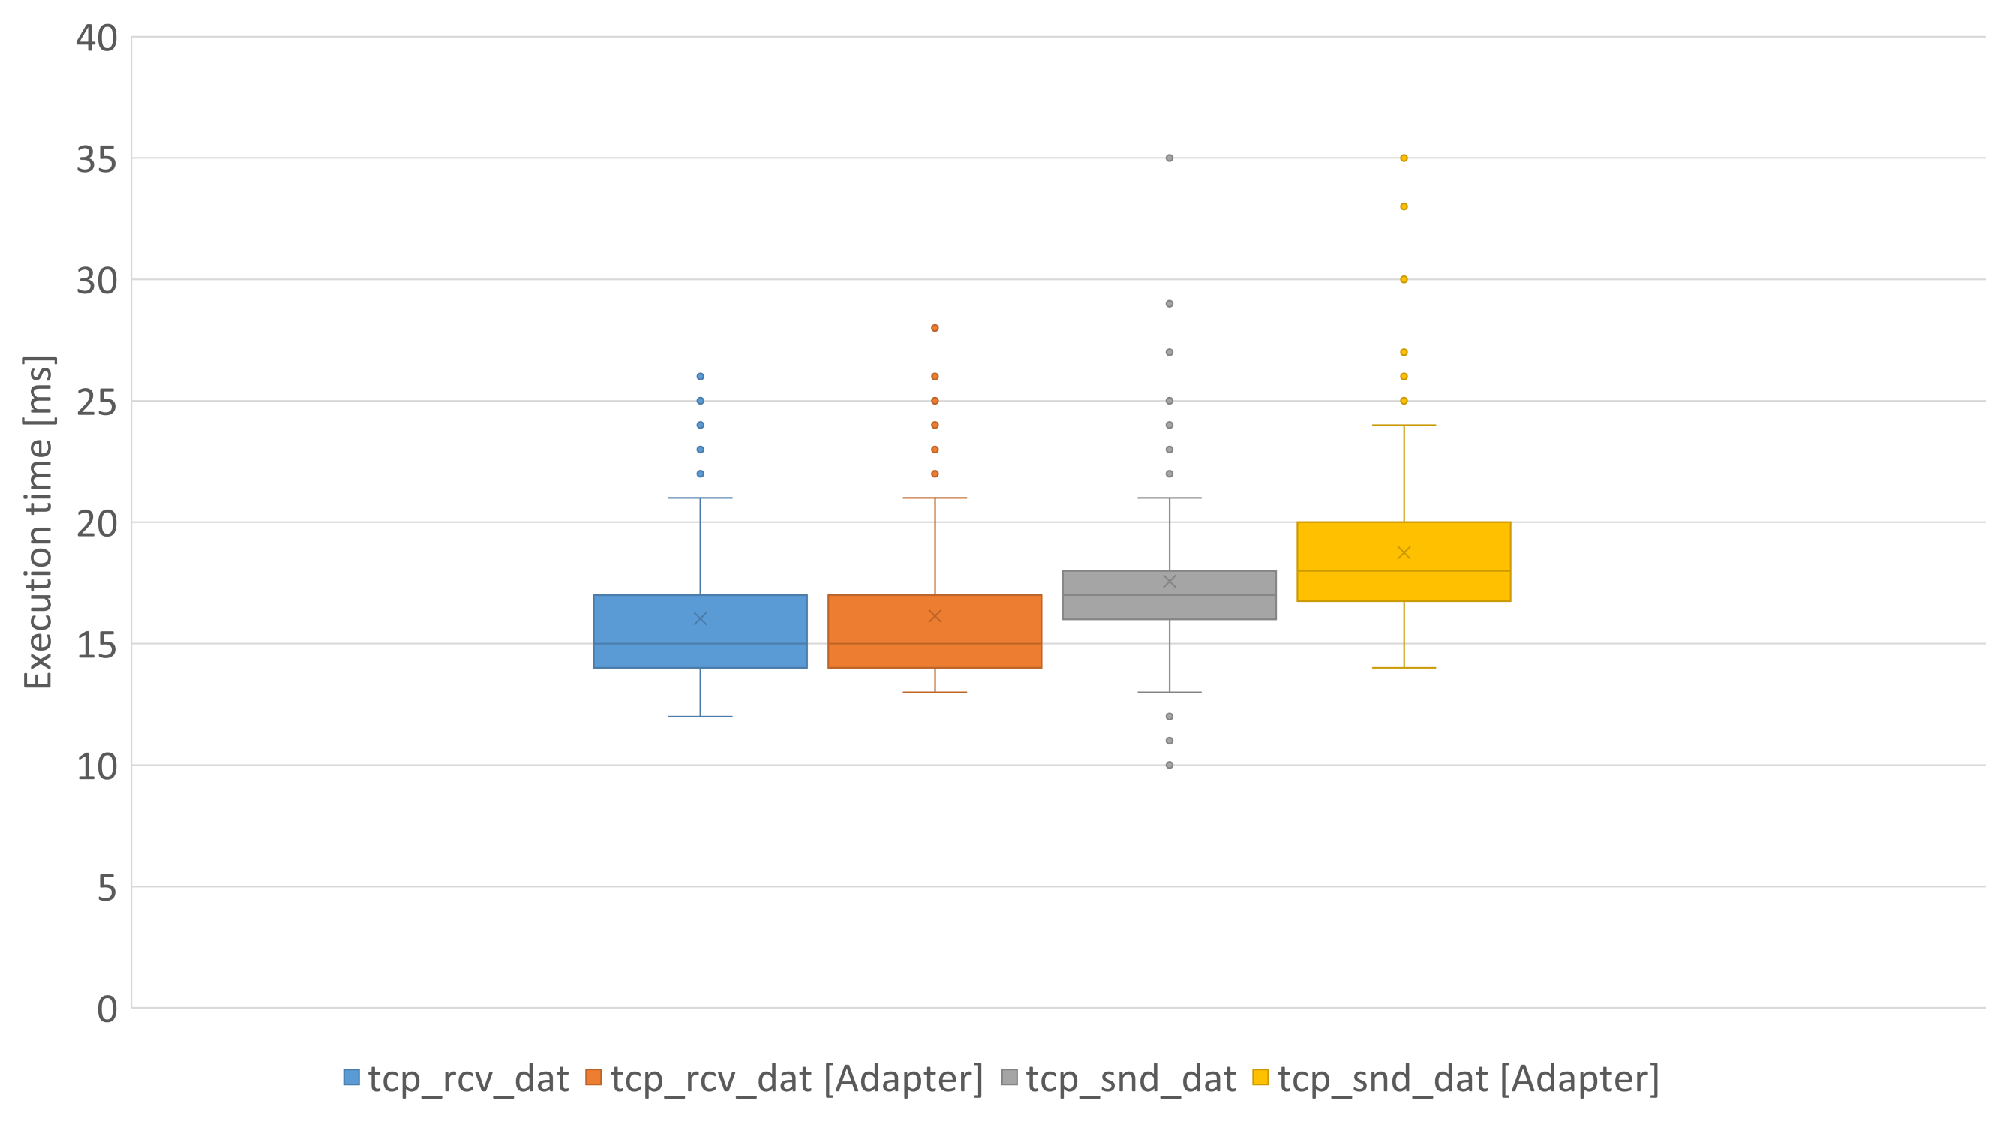
\includegraphics[width=8.0cm,clip]{figure/EvaluationOfAdapter.pdf}
    \caption{Execution times in two cases (without/with TECS adapter)}
    \label{fig:EvaluationOfAdapter}
\end{figure}


\section{Related Work}
\label{sec:Related Work}

Open-source TCP/IP protocol stacks for embedded systems have been developed such uIP \cite{par:uIP}, lwIP \cite{par:lwIP}.

{\bf uIP:}
uIP (microIP) is a very small TCP/IP stack intended for tiny 8- and 16-bit microcontrollers.
uIP requires only about 5 KB of code size and several hundred bytes of RAM.
uIP has been ported to various systems and has found its way into many commercial products.
Following the release of ver. 1.0, later versions of uIP, including uIPv6, have been integrated with Contiki OS \cite{par:Contiki},\cite{url:Contiki}, an operating system to connect tiny microcontrollers to the Internet.

{\bf lwIP:}
lwIP (lightweightIP) is a small TCP/IP implementation for embedded systems that is intended to reduce memory resource usage while still maintaining a full-scale TCP.
lwIP requires about 40 KB of ROM and tens of KB of RAM.
lwIP is larger than uIP, but provides better throughput.

% {\bf CiAO/IP:}
% \\
% \\
% Should be written
% \\
% \\

\section{Conclusion}
\label{sec:Conclusion}

This paper proposed TINET+TECS, a component-based TCP/IP protocol stack for embedded systems.
TINET+TECS is a componentized version of TINET, a compact TCP/IP protocol stack that uses TECS.
Because TINET comprises many macros and complicated codes, its software productivity is low.
The proposed framework improves on TINET's configurability while suppressing the overhead of componentization.
Scalability is also improved because the component-based framework simplifies to add/remove and change protocols such as TCP/UDP, IPv4/IPv6, and Ethernet/PPP.

This paper also presented dynamic connection, a new TECS method, to enable dynamic processing while reducing memory consumption.
TINET+TECS utilizes dynamic connection to satisfy the TINET specification for supporting static generation of CEPs and REPs.
As the TECS adapter supports legacy codes, existing TCP/IP applications can run without modification in the proposed framework.

In future work, we will adapt the proposed framework to cooperate with mruby on TECS \cite{par:mrubyonTECS} to more easily manage IoT devices.
Note that mruby is a scripting language for embedded systems \cite{par:mruby}.
We will support functionalities in which TINET functions can be utilized from mruby programs as an extension of mruby-socket \cite{url:mruby-library}.
    
% conference papers do not normally have an appendix


% use section* for acknowledgment
\section*{Acknowledgment}

The authers would like to thank Hiroaki Nagashima for supporting this research.
This work is supported by JSPS KAKENHI Grant Number 15H05305.

% trigger a \newpage just before the given reference
% number - used to balance the columns on the last page
% adjust value as needed - may need to be readjusted if
% the document is modified later
%\IEEEtriggeratref{8}
% The "triggered" command can be changed if desired:
%\IEEEtriggercmd{\enlargethispage{-5in}}

% references section
\bibliographystyle{IEEEtranBST2/IEEEtran}
\bibliography{ref}

% that's all folks
\end{document}
